\documentclass[twoside]{article}

\usepackage{graphicx}
\usepackage[a4paper, total={6.6in, 9.6in}, includehead]{geometry}
\usepackage[T1]{fontenc}
\usepackage[french]{babel}
\usepackage{hyphenat}
\usepackage{fancybox}
\usepackage{fancyhdr}
\hyphenation{mate-mática recu-perar}
\usepackage{pifont}
\usepackage{tikz,tikz-3dplot}
\usepackage{listings}
\usepackage{etoolbox}
\usepackage{lmodern}
% \usepackage[dvipsnames]{xcolor}
\usetikzlibrary{shapes.geometric}
\usetikzlibrary{shapes.symbols}
\usetikzlibrary{decorations.pathreplacing}
\usepackage{caption}
\usepackage{subcaption}
\usepackage{cprotect}
\usepackage{tabularx}
\usepackage{pdfpages}
\usepackage{lastpage}
\usepackage{titlesec}
\usepackage{hyperref}
\usepackage{dirtree}
\usepackage{wrapfig}
\usepackage{lipsum}
\usepackage{cancel}
\usepackage{chngcntr}
\usepackage{amsmath}


\newlength{\larg}
\setlength{\larg}{15.5cm}
\renewcommand{\footrulewidth}{0.4pt}

\definecolor{font}{RGB}{28, 28, 28}
\definecolor{codegray}{rgb}{0.5,0.5,0.5}
\definecolor{A}{RGB}{245, 87, 146}
\definecolor{B}{RGB}{242, 142, 93}
\definecolor{C}{RGB}{245, 206, 60}
\definecolor{D}{RGB}{159, 210, 108}
\definecolor{E}{RGB}{110, 210, 222}
\definecolor{F}{RGB}{161, 147, 232}
\definecolor{G}{RGB}{85, 83, 88}


\renewcommand*{\lstlistlistingname}{Liste des codes}
\renewcommand*{\lstlistingname}{Code}
\lstdefinestyle{terminal}{
    postbreak=\mbox{{$\hookrightarrow$}\space},
    aboveskip=1.5em,
    belowskip=1.5em,
    escapeinside={(*@}{@*)},
    breaklines=true,
    frame=tb,
    numbers=none,
    inputencoding=utf8,  % Input encoding
    extendedchars=true,  % Extended ASCII
    literate={
        {á}{{\'a}}1  {é}{{\'e}}1  {í}{{\'i}}1 {ó}{{\'o}}1  {ú}{{\'u}}1
        {Á}{{\'A}}1  {É}{{\'E}}1  {Í}{{\'I}}1 {Ó}{{\'O}}1  {Ú}{{\'U}}1
        {à}{{\`a}}1  {è}{{\`e}}1  {ì}{{\`i}}1 {ò}{{\`o}}1  {ù}{{\`u}}1
        {À}{{\`A}}1  {È}{{\'E}}1  {Ì}{{\`I}}1 {Ò}{{\`O}}1  {Ù}{{\`U}}1
        {ä}{{\"a}}1  {ë}{{\"e}}1  {ï}{{\"i}}1 {ö}{{\"o}}1  {ü}{{\"u}}1
        {Ä}{{\"A}}1  {Ë}{{\"E}}1  {Ï}{{\"I}}1 {Ö}{{\"O}}1  {Ü}{{\"U}}1
        {â}{{\^a}}1  {ê}{{\^e}}1  {î}{{\^i}}1 {ô}{{\^o}}1  {û}{{\^u}}1
        {Â}{{\^A}}1  {Ê}{{\^E}}1  {Î}{{\^I}}1 {Ô}{{\^O}}1  {Û}{{\^U}}1
        {œ}{{\oe}}1  {Œ}{{\OE}}1  {æ}{{\ae}}1 {Æ}{{\AE}}1  {ß}{{\ss}}1
        {ç}{{\c c}}1 {Ç}{{\c C}}1 {ø}{{\o}}1  {Ø}{{\O}}1   {å}{{\r a}}1
        {Å}{{\r A}}1 {ã}{{\~a}}1  {õ}{{\~o}}1 {Ã}{{\~A}}1  {Õ}{{\~O}}1
        {ñ}{{\~n}}1  {Ñ}{{\~N}}1  {¿}{{?`}}1  {¡}{{!`}}1
        {°}{{\textdegree}}1 {º}{{\textordmasculine}}1 {ª}{{\textordfeminine}}1
    }
}
\lstdefinestyle{prog}{
    language=C,
    basicstyle=\ttfamily\small,
    stepnumber=1,                   
    numbersep=5pt,
    numberstyle=\tiny\color{codegray},
    postbreak=\mbox{{$\hookrightarrow$}\space},
    showstringspaces=false,
    aboveskip=1.5em,
    belowskip=1.5em,
    % escapechar=\&,
    escapeinside={(*@}{@*)},
    breaklines=true,
    frame=tb,
    numbers=left,
    showlines=true,
    consecutivenumbers=false,
    texcl=true,
    % identifierstyle={\color{B}},
    % backgroundcolor={\color{font}},
    keywordstyle={\color{A}},
    stringstyle={\color{D}},
    commentstyle={\color{G}},
    emph={[1]=, <, >, +, -, /, //, *}, emphstyle={[1]\color{A}},
    emph={[5]void, uint32_t, uint16_t, uint8_t, size_t, bool, float}, emphstyle={[5]\color{E}},
    % otherkeywords={\&},
    % emph={&},
    % emph={[6]True, False, None}, emphstyle={[6]\color{F}},
    inputencoding=utf8,  % Input encoding
    extendedchars=true,  % Extended ASCII
    literate={
        {á}{{\'a}}1  {é}{{\'e}}1  {í}{{\'i}}1 {ó}{{\'o}}1  {ú}{{\'u}}1
        {Á}{{\'A}}1  {É}{{\'E}}1  {Í}{{\'I}}1 {Ó}{{\'O}}1  {Ú}{{\'U}}1
        {à}{{\`a}}1  {è}{{\`e}}1  {ì}{{\`i}}1 {ò}{{\`o}}1  {ù}{{\`u}}1
        {À}{{\`A}}1  {È}{{\'E}}1  {Ì}{{\`I}}1 {Ò}{{\`O}}1  {Ù}{{\`U}}1
        {ä}{{\"a}}1  {ë}{{\"e}}1  {ï}{{\"i}}1 {ö}{{\"o}}1  {ü}{{\"u}}1
        {Ä}{{\"A}}1  {Ë}{{\"E}}1  {Ï}{{\"I}}1 {Ö}{{\"O}}1  {Ü}{{\"U}}1
        {â}{{\^a}}1  {ê}{{\^e}}1  {î}{{\^i}}1 {ô}{{\^o}}1  {û}{{\^u}}1
        {Â}{{\^A}}1  {Ê}{{\^E}}1  {Î}{{\^I}}1 {Ô}{{\^O}}1  {Û}{{\^U}}1
        {œ}{{\oe}}1  {Œ}{{\OE}}1  {æ}{{\ae}}1 {Æ}{{\AE}}1  {ß}{{\ss}}1
        {ç}{{\c c}}1 {Ç}{{\c C}}1 {ø}{{\o}}1  {Ø}{{\O}}1   {å}{{\r a}}1
        {Å}{{\r A}}1 {ã}{{\~a}}1  {õ}{{\~o}}1 {Ã}{{\~A}}1  {Õ}{{\~O}}1
        {ñ}{{\~n}}1  {Ñ}{{\~N}}1  {¿}{{?`}}1  {¡}{{!`}}1
        {°}{{\textdegree}}1 {º}{{\textordmasculine}}1 {ª}{{\textordfeminine}}1
        % {0}{{{\color{F}0}}}1
        % {1}{{{\color{F}1}}}1 {2}{{{\color{F}2}}}1 {3}{{{\color{F}3}}}1
        % {4}{{{\color{F}4}}}1 {5}{{{\color{F}5}}}1 {6}{{{\color{F}6}}}1
        % {7}{{{\color{F}7}}}1 {8}{{{\color{F}8}}}1 {9}{{{\color{F}9}}}1
        {=}{{{\color{A}$=$}}}1
        {==}{{{\color{A}$=\joinrel=$}}}1
        {<=}{{{\color{A}$\leq$}}}1
        {>=}{{{\color{A}$\geq$}}}1
        {!=}{{{\color{A}$\neq$}}}1
        {:=}{{{\color{A}:=}}}1
    }
}



\titleclass{\subsubsubsection}{straight}[\subsection]

\newcounter{subsubsubsection}[subsubsection]
\renewcommand\thesubsubsubsection{\thesubsubsection.\arabic{subsubsubsection}}
\renewcommand\theparagraph{\thesubsubsubsection.\arabic{paragraph}} % optional; useful if paragraphs are to be numbered

\titleformat{\subsubsubsection}
  {\normalfont\normalsize\bfseries}{\thesubsubsubsection}{1em}{}
\titlespacing*{\subsubsubsection}
{0pt}{3.25ex plus 1ex minus .2ex}{1.5ex plus .2ex}



\title{
    \Huge \textbf{Documentation de OMEGAAA} \\
    \large \textbf{O}rdinateur de \textbf{M}esure, d'\textbf{E}valuation, de \textbf{G}estion\\
    \large et d'\textbf{A}nalyse pour l'\textbf{A}éronautique et l'\textbf{A}érospatiale\\
}
\date{\today}
\author{Alexis Paillard}  

\makeatletter
\newcommand\footnoteref[1]{\protected@xdef\@thefnmark{\ref{#1}}\@footnotemark}
\def\toclevel@subsubsubsection{4}
\def\l@subsubsubsection{\@dottedtocline{4}{7em}{4em}}
\def\@maketitle{
    % \begin{center}
    % \begin{tabular}{>{\raggedright\arraybackslash}m{0.5\textwidth}
    %     >{\raggedleft\arraybackslash}m{0.5\textwidth}}
    %     
\includegraphics[width=0.25\textwidth]{image/Logo_Alpha2.png} & {logo de Gaïa}
    % \end{tabular}
    % \begin{tabular}{m{0.6\textwidth}m{0.4\textwidth}}
    %     AeroIPSA & Gaïa
    % \end{tabular}
    % \end{center}
    \begin{flushright}
        {\rule{\larg}{1mm}}\\
        \vspace{3mm}
        \@title
        \vspace{2mm}
        {\rule{\larg}{1mm}}\\
    \end{flushright}
    \vspace{1cm}
    \begin{figure}[h]
        \centering
        \caption{Logo du projet OMEGAAA}
    \end{figure}
    \vfill
    \begin{tabular}{>{\raggedright\arraybackslash}m{0.5\textwidth}
        >{\raggedleft\arraybackslash}m{0.5\textwidth}}
        \@author & \@date \\
        \hline
    \end{tabular}
}
\makeatother

\setcounter{secnumdepth}{4}
\setcounter{tocdepth}{4}

\counterwithin{figure}{section}
\AtBeginDocument{\numberwithin{lstlisting}{section}}


\begin{document}


\pagenumbering{gobble}
\maketitle

\newpage

\pagestyle{fancy}
\fancyhead{}\fancyfoot{} % clear all fields
\fancyhead[L]{\textbf{Documentation d l'OMEGAAA}}
\fancyhead[R]{\textbf{AeroIPSA}}
\fancyfoot[L]{Alexis Paillard}
\fancyfoot[R]{\thepage/\pageref{LastPage}}

\newpage
\pagenumbering{arabic}
\setcounter{page}{2}

\fancyhead{}\fancyfoot{} % clear all fields
\fancyhead[RO]{\textbf{Documentation d l'OMEGAAA}}
\fancyhead[LE]{\textbf{AeroIPSA}}
\fancyfoot[L]{Alexis Paillard}
\fancyfoot[R]{\thepage/\pageref{LastPage}}

\tableofcontents
\newpage

\listoffigures
\lstlistoflistings
\newpage

% \setcounter{page}{1}
\section*{Mise en contexte}
\addcontentsline{toc}{section}{\protect\numberline{}Mise en contexte}

Ce document a pour but de présenter l'OMEGAAA, un concepte d'ordinateur de bord
pour une fusée amateur. Le projet a été mené par Alexis Paillard et se base en
majeur partie sur le projet Unknown réalisé dans le cadre de l'association
AeroIPSA.\\

\subsection*{- AeroIPSA}
AéroIPSA est une association étudiante de l'école d'ingénieurs IPSA qui conçoit et
réalise entièrement des projets fonctionnels en rapport avec le secteur
aérospatial. Elle rassemble des étudiants autour de projets d'astromodélisme,
principalement de lanceurs, mais aussi de Cansats (micro-satellites atmosphérique).
Cela permet aux différents membres de l'association d'appliquer les notions
apprises durant leur cursus au profit d'un projet d'envergure et d'acquérir les
compétences nécessaires dans leur futur métier d'ingénieur.\\

\subsection*{- Unknown}
Unknown est un projet de module électronique de fusée expérimentale réalisé par
Vincent Fauquembergue et Alexis Paillard. Les expériences du projet Unknown ont été
les suivantes :
\begin{itemize}
    \item \textbf{Expérience principale} : Relocaliser une fusée après son lancement
    grâce à un module de télémesure LoRa renvoyant les données GNSS tout au long du
    vol.
    \item \textbf{Expérience secondaire} : Réalisation d'une collecte de données
    provenant de nombreux capteurs, barométrique et centrale inertielle, afin de
    reconstituer le vol après récupération des données stockées sur une mémoire
    flash.
\end{itemize}
L'un des objectifs du projet Unknown était de réaliser un module électronique se
voyant plus facilement intégrable dans une fusée amateur. Cela s'est traduit par
l'utilisation d'une seule carte électronique ayant tous ses composants directement
soudés dessus ainsi que l'utilisation d'un microcontrôleur autre que l'Arduino ou
que la Teensy. Le choix fait s'est porté sur un STM32F4 de STMicroelectronics. La
programmation de ce microcontrôleur a été réalisée en C et un bon nombre des
drivers nécessaires ont dû être réadapté par les membres du projet ce qui a permis
d'acquérir de nouvelles compétences en programmation bas niveau.

L'annexe \ref{anx:unknown} présente le rapport du projet Unknown ainsi que des
photos du module.

\subsection*{- OMEGAAA}
OMEGAAA est l'acronyme de \textbf{O}rdinateur de \textbf{M}esure,
d'\textbf{E}valuation, de \textbf{G}estion et d'\textbf{A}nalyse pour
l'\textbf{A}éro-nautique et l'\textbf{A}érospatiale. Il s'agit d'un concepte
d'ordinateur de bord qui a pour but de gérer les différentes phases de vol d'une
fusée amateur, tout en effectuant des mesures notamment d'accélérations et de
vitesses de rotation (à l'aide d'un IMU). Ces données sont ensuite traitées pour en
extraire la position et l'attitude de la fusée et enregistrées dans une mémoire.
L'OMEGAA gère également une communication par télémétrie avec une station au sol.

Ce module fait suite au projet Unknown en reprenant les composants électroniques de
ce dernier. Il a pour but de continuer à développer les compétences en
programmation acquises lors du projet Unknown et d'en développer de nouvelle comme
la création du RTOS \footnote{Un RTOS (\textbf{R}eal \textbf{T}ime
\textbf{O}perating \textbf{S}ystem)  est un système d'exploitation conçu pour gérer
les ressources matérielles de manière à garantir que des tâches critiques soient
exécutées parallèlement à d'autre et dans des délais stricts et prévisibles.
Ce type de système est laregement employé dans des application tels que les systèmes
embarqués, les dispositifs médicaux, les systèmes de contrôle industriel, et les
applications aéronautiques et aérospatiales...}. Cet ordinateur de bord étant
fictif, il n'a pas été réalisé mais l'ensemble des travaux et des recherches
effectuées pour sa conception sont présentées dans ce document et ont pour but de
servir de support pour la réalisation d'un tel module électronique.\\

\newpage
\section{Objectifs}

L'objectif de l'OMEGAAA est d'avoir un ordinateur de bord relativement puissant
mais également polyvalant. Afin de démontrer les capacités de l'OMEGAAA, les
objectifs suivants ont été fixés. L'OMEGAAA doit être capable :

\begin{itemize}
    \item D'acquérir des données de divers capteurs.
    \item D'effectuer des calculs sur les données acquises.
    \item De stocker bons nombres de données.
    \item De communiquer avec l'extérieur par radio.
    \item D'aborder différents comportements en fonction de
          l'état de la fusée.
    \item D'effectuer l'ensemble de ces tâches en optimisant
          les temps de processuces.\\
\end{itemize}

Le logigramme suivant présente les 5 étapes principales qu'une fusée peut avoir.
L'algorithme générale du programme de l'OMEGAAA est alors présenté. A noter que
le schéma ne fait qu'exposer brievement la logique du programme et n'est pas
exhaustif.

\begin{figure}[h]
    \centering
    \tikzstyle{line} =[very thick, rounded corners=5pt]
\tikzstyle{arrow}=[line, ->, >=latex]

\tikzstyle{size}=[minimum width=2cm, minimum height=1cm]
\tikzstyle{bx}=[draw, size, align=center]

\tikzstyle{actionbx}=[bx, rounded corners=5pt]
\tikzstyle{logbx}   =[bx, rounded corners=5pt, minimum width=6cm]
\tikzstyle{objbx}   =[bx]
\tikzstyle{onoffbx} =[bx, ellipse]
\tikzstyle{ifelsebx}=[bx, diamond, aspect=2.5]
\tikzstyle{fluxbx}  =[draw, diamond, aspect=1, minimum width=1cm, minimum height=1cm]
\tikzstyle{inbx}    =[bx, signal , signal from=west   , signal to=nowhere]
\tikzstyle{outbx}   =[bx, signal , signal from=nowhere, signal to=east]

\begin{tikzpicture}[scale=1]
    \node[onoffbx]  (A) at ( 0.0, +1.3) {Début};
    \node[actionbx] (B) at ( 0.0, +0.0) {Initialisation\\composants};
    \node[actionbx] (C) at ( 0.0, -1.4) {Initialisation\\communication LoRa};
    \node[actionbx] (D) at (-2.5, -3.5) {Attente\\commande armement\\séquence vol};
    \node[actionbx] (E) at (-2.5, -5.5) {Attente\\détection lancement};

    \node[logbx, rotate=90] (log) at ( 2.5, -5.6) {Envoie de messages d'informations\\de l'état de l'OMEGAAA par LoRa};
    
    \node[actionbx] (F) at (-2.5, -7.5) {Mesure\\Analyse/traitement\\Enregistrement\\Envoie par LoRa};
    \draw[dotted, thick] (-4.1, -7.06) -- (-0.9, -7.06);
    \draw[dotted, thick] (-4.1, -7.50) -- (-0.9, -7.50);
    \draw[dotted, thick] (-4.1, -7.93) -- (-0.9, -7.93);
    
    \node[ifelsebx] (H) at (-2.5, -9.6) {Atterri ?};

    \node[actionbx] (I) at (-2.5, -11.3) {Gestion consommation\\allégées};
    \node[actionbx] (J) at (+1.5, -11.3) {Envoie par LoRa\\de la position GPS};
    
    \node[ifelsebx] (K) at (5, -11.3) {Récupéré ?};

    \node[actionbx] (L) at (2.0, -12.7) {Envoie des données \\ enregistrées};

    \node[onoffbx]  (M) at (-1.0, -12.7) {Fin};

    \draw[arrow] (A)  -- (B);
    \draw[arrow] (B)  -- (C);
    \draw[arrow] (C) |- (-1, -2.2) -| (D);
    \draw[arrow] (C) |- (+1, -2.2) -| (log);

    \draw[arrow] (D) -| (-4.75, -3.5) |- (-3.5, -2.30) -| (D);
    \draw[arrow] (D) -- (E);

    \draw[arrow] (E) -| (-4.75, -5.0) |- (-3.5, -4.5) -| (E);

    \draw[arrow] (E) -- (F);
    \draw[arrow] (F) -- (H);
    \draw[arrow] (H) -- ++(2.5, 0) node[pos=0.5, above] {Non} -| ++(0, 1) |- ++(-1, 2.35) -| (F);
    \draw[arrow, dotted] (log) |- ++(-1, -3.15) -| (H);
    \draw[arrow, dotted] (H) -| ++(6.25, 2) |- ++(-1, 5.35) -| (log);

    \draw[arrow] (H) -- (I) node[pos=0.5, left] {Oui};
    \draw[arrow] (I) -- (J);
    \draw[arrow] (J) -- (K);
    \draw[arrow] (K) |- ++(-1, 0.85) node[pos=0.5, right] {Non} -| ++(-4.45, -0.85) |- (J);

    \draw[arrow] (K) |- (L) node[pos=0.3, right] {Oui};
    \draw[arrow] (L) -- (M);

    \draw[dashed, very thick] (-6, -2.00) -- (6, -2.00);
    \draw[dashed, very thick] (-6, -6.15) -- (1, -6.15);
    \draw[dashed, very thick] (-6, -10.2) -- (6, -10.2);
    \draw[dashed, very thick] (-6, -12.0) -- (6, -12.0);
    
    \draw[color=red] (-5,   0.00) node[above, rotate=90] {Initialisation};
    \draw[color=red] (-5,  -4.00) node[above, rotate=90] {Prévol};
    \draw[color=red] (-5,  -8.25) node[above, rotate=90] {Vol};
    \draw[color=red] (-5, -11.10) node[above, rotate=90] {Postvol};
    \draw[color=red] (-5, -13.00) node[above           ] {Récupération};

\end{tikzpicture}
    \caption{Logigramme du programme de l'OMEGAAA}
\end{figure}


\newpage
\section{Projet STM}

Le programme de l'OMEGAAA est écrit à l'aide de l'environnement de développement
STMicroelectronics. Ce dernier permet de créer des projets pour les microcontrôleurs
de la firme. Chaque projets est composé de plusieurs sous-dossiers et fichiers. Le
HAL\footnote{HAL (pour \textbf{H}ardware \textbf{A}bstraction \textbf{L}ayer) est
une bibliothèque logicielle qui fournit une interface de programmation pour les
périphériques matériels.} fournit par STMicroelectronics étant écrit en C, et que
bons nombres d'information, tutoriels et exemples sont disponibles en C, le programme
de l'OMEGAAA utilisera ce language.


\begin{minipage}{0.95\textwidth}
    \begin{wrapfigure}{L}{0.35\textwidth}
    \vspace{-1.0cm}
    \dirtree{%
    .1 ....
    .1 Core.
        .2 Inc.
            .3 ....
        .2 Src.
            .3 drivers.
                .4 BMI088.c.
                .4 BMP388.c.
                .4 buzzer.c.
                .4 gps.c.
                .4 rfm96w.c.
                .4 w25q\_mem.c.
                .4 ....
            .3 peripherals.
                .4 dma.c.
                .4 gpio.c.
                .4 i2c.c.
                .4 spi.c.
                .4 tim.c.
                .4 usart.c.
                .4 ....
            .3 flash\_stream.c.
            .3 main.c.
            .3 scheduler.c.
            .3 tools.c.
            .3 ....
            .3 stm32f4xx\_hal\_msp.c.
            .3 stm32f4xx\_it.c.
            .3 syscalls.c.
            .3 sysmem.c.
            .3 system\_stm32f4xx.c.
    .1 ....
    }
    \caption{Arboressance du programme}
    \end{wrapfigure}
    
    \vspace{1.0cm}
    
    L'intégralité du programme de l'OMEGAAA se trouve dans le dossier
    "\texttt{Core}". Ce dernier est composé des fichiers de déclarations (.h) dans
    le dossier \texttt{Inc} et des fichiers de programme (.c) dans le dossier
    \texttt{Src}. Tous     les programmes relatifs aux composants externes au
    microcontrôleur (capteurs, ...) se trouve dans le dossier \texttt{drivers} et
    ceux relatifs à la gestion des composants internes (gestionnaires des
    périphériques, ...) dans \texttt{peripherals}.
    
    \vspace{0.5cm}
    
    On retrouve dans le dossier \texttt{Inc} symétriquement la même arboressance de
    dossiers et fichiers que dans le dossier \texttt{Src} à l'extention près (non
    des "\texttt{.c}" mais des "\texttt{.h}").
    
    \vspace{0.5cm}
    
    Le point d'entrée du programme se trouve dans la fonction \texttt{main} du
    fichier du même nom.
    
    
    \vspace{0.2cm}
    Le fichier \texttt{scheduler.c} contient l'implémentation de l'ordonanceur et
    la définition d'une tâche (cf. \ref{subsec:implementation}).

    
    \vspace{0.2cm}
    Le fichier \texttt{flash\_stream.c} contient les structures et fonctions
    permettant de lire et d'écrire des données dans une mémoire tout en gérant
    les pointeurs de lecture et d'écriture.

    
    \vspace{0.2cm}
    Le fichier \texttt{tools.c} contient des fonctions utilisées à différents
    endroits du programme.

    \vspace{0.5cm}

    Enfin, les fichiers \texttt{stm32f4xx\_hal\_msp.c},
    \texttt{stm32f4xx\_it.c}, \texttt{syscalls.c}, \texttt{sysmem.c} et
    \texttt{system\_stm32f4xx.c} sont des fichiers de configuration,
    de gestion des interruptions, de gestion de la mémoire et de gestion
    du système général du microcontrôleur. Ces fichiers sont générés
    automatiquement par l'environnement de développement et bien qu'ils le
    peuvent, ils ne seront pas modifiés par l'utilisateur.
    
\end{minipage}
\newpage
\section{Composants externes}
\label{sec:drivers}

Cette section présente les divers composants électroniques utilisés dans le projet OMEGAAA
ainsi que leur driver associé.

\subsection{Vue d'ensemble}

L'OMEGAAA possède plusieurs composants que l'ont peut regrouper en quatre
catégories en plus du microcontroleur : les capteurs, les composants de stockage,
les témoins et les composants de communication.\\

Le microcontroleur est le cerveau de l'OMEGAAA. Il possède le programme
informatique, les moyens pour l'exécuter et gérer les autres composants électroniques.
l'un des concepts clé utilisé dans le microcontroleur est sa capacité à effectuer des
échanges d'informations entre les composants par DMA \footnote{DMA : \textbf{D}irect
\textbf{M}emory \textbf{A}cces. Avec la communication par DMA, le microcontrôleur
peut déléguer la tâche de transfert de données à un contrôleur DMA dédié. Le contrôleur
DMA est capable de transférer les données directement entre les périphériques (par exemple,
entre un capteur) et la mémoire de l'ordinateur sans passer par le CPU. Cela libère le
temps CPU pour qu'il puisse effectuer d'autres tâches.}. Le projet OMEGAAA se base sur
l'utilisation d'un STM32F411CEx.\\

Les différents capteurs sont :
\begin{itemize}
    \item Un IMU (Inertial Measurement Unit) qui mesure l'accélération de
    translation et la vitesse de rotation de la fusée (ref: BMI088).
    \item Un GPS qui mesure la position de la fusée et sa vitesse (ref: MAX-M10Q).
    \item Un baromètre qui mesure l'altitude de la fusée et un thermomètre.
    (ref: BMP388).\\
\end{itemize}

\begin{minipage}{0.95\textwidth}

    \begin{wrapfigure}{R}{0.5\textwidth}
        \vspace{1.4cm}
        \centering
        \begin{tikzpicture}[scale=1.2]
    
            \node[draw, rectangle, minimum width=1cm, minimum height=1cm, fill=gray!80, rounded corners]      (micro) at (0, 0) {$\mu C$\footnotemark};
            \node[draw, rectangle, minimum width=2.0cm, minimum height=1.75cm, fill=gray!20, rounded corners] (imu)   at (2.25, +0.60) {};
            \node[draw, rectangle, minimum width=0.5cm, minimum height=0.5cm, fill=white, rounded corners]    (acc)   at (2.25, +0.75) {\tiny Accelerometer};
            \node[draw, rectangle, minimum width=0.5cm, minimum height=0.5cm, fill=white, rounded corners]    (gry)   at (2.25, +0.25) {\tiny Gyroscope};
            \node at (2.25, +1.10) {IMU};
            \node[draw, rectangle, minimum width=1cm, minimum height=1cm, fill=gray!20, rounded corners]      (gps)   at (0, +1.50) {GPS};
            \node[draw, rectangle, minimum width=2.0cm, minimum height=1.60cm, fill=gray!20, rounded corners] (bmu)   at (-2.25, +0.00) {};
            \node[draw, rectangle, minimum width=0.5cm, minimum height=0.5cm, fill=white, rounded corners]    (bar)   at (-2.25, +0.25) {\tiny Barometer};
            \node[draw, rectangle, minimum width=0.5cm, minimum height=0.5cm, fill=white, rounded corners]    (tem)   at (-2.25, -0.25) {\tiny Thermometer};
            \node[draw, rectangle, minimum width=1cm, minimum height=1cm, fill=gray!20, rounded corners]      (tel)   at (+2.00, -1.20) {Telem.};
            \node[draw, rectangle, minimum width=1cm, minimum height=1cm, fill=gray!20, rounded corners]      (mem)   at (-1.55, -1.20) {Flash};
            \node[draw, rectangle, minimum width=1cm, minimum height=1cm, fill=gray!20, rounded corners]      (buz)   at (-1.25, +1.30) {Buzzer};
    
            \draw[<->] (micro) -| ++(1, 0.25) |- (imu);
            \draw[<->] (micro) -- (gps);
            \draw[<->] (micro.-150) -| ++(-0.75, 0.2) |- (bmu);
            \draw[<->] (micro) -| ++(1, -0.25) |- (tel);
            \draw[<->] (micro) |- (mem);
            \draw[->] (micro.160) -| (buz.-55);
    
            \node at (+0.75, 0.15) {\tiny SPI 1};
            \node at (-0.70, -0.35) {\tiny I2C};
            \node at (+0.35, 0.75) {\tiny UART};
            \node at (-0.70, 0.55) {\tiny TIM\footnotemark};
            \node at (+0.35, -0.65) {\tiny SPI 2};
    
        \end{tikzpicture}
        \caption{Schéma des composants de l'OMEGAAA}
        \label{fig:omega}
    \end{wrapfigure}

Un seul composant de stockage est utilisé : une mémoire flash de 16 Mo
(ref: W25Q128JVPQ).

\vspace{0.5cm}

Les témoins sont des composants qui permettent de savoir dans quel état se
trouve l'OMEGAAA. Ils peuvent être sonores ou lumineux. Dans la version actuelle
de l'OMEGAAA, un buzzer passif est utilisé permettant la création de mélodie.

\vspace{0.5cm}

Un seul composant de communication est utilisé, un module de télémétrie par
protocole et modulation LoRa (ref: RFM98W). A noté que le microcontroleur
possède aussi des moyens de communocation interfaçable avec un ordinateur (via
USB).

\vspace{0.5cm}

Un cinquième type de composant pourrait être ajouté : les actionneurs. Ils
permetteraient d'agire physiquement sur des éléments de la fusée. Par exemple,
un servomoteur contrôlant une surface portante.

\end{minipage}

\vspace{0.5cm}

La figure \ref{fig:omega} montre un schéma des composants de l'OMEGAAA et
leurs interconnexions. Les flèches indiquent les protocoles de communication
utilisés entre les composants.\\


\footnotetext{$\mu C$ : \textbf{M}icro\textbf{C}ontroleur.}
\footnotetext{TIM : \textbf{T}imer \textbf{I}nterface \textbf{M}odule sert dans ce contexte à générer des signaux PWM.}
\newpage
\subsection{Communication entre composants}

% \subsubsection{Problématique et logique de communication}

La programmation des protocoles de communications entre les différents composants
électroniques dans un système temps réel se révèle être un éléments clé pour le bon
fonctionnement de ce dernier mais aussi ardu à mettre en place. Il n'est par exemple
pas souhaitable de bloquer certaines tâches du système lors de la transmission ou
de la réception de données entre les composants. C'est notamment pour cela que le
choix d'un microcontrôleur contre un microprocesseur a été fait. En effet, un
microcontrôleur est capable de gérer des interruptions matérielles bien plus
facilement et efficacement qu'un microprocesseur seul grâce aux périphériques
intégrés de ce premier. Néanmoins une vigilent plus importante comparé à un
système séquentiel est nécessaire. En effet, il est possible de se retrouver avec
des problèmes de synchronisation entre les différents composants électroniques. Il
faut ainsi être capable de ne pas permettre à deux tâches d'intéragir avec des
composants utilisant le même bus de communication en même temps.\\

\subsubsection{Présentation du concepte}

Prenons l'exemple d'une communication SPI. Il est possible de partager un bus SPI
entre plusieurs composants électroniques. Cependant, il est nécessaire de s'assurer
que le bus SPI soit bien libre avant de pouvoir transmettre ou recevoir des données.
Voici l'implémentation de quelques outils permettant de gérer la communication SPI
de manière asynchrone.

\begin{lstlisting}[style=prog, frame=shadowbox, caption={Définition des outlis spi suplémentaires (tools.h)}, label={lst:tools_h},
    emph={[1]SPI_HandleTypeDef_flag_init, ASYNC_SPI_TxRx_DMA_init, ASYNC_SPI_TxRx_DMA, add_task, kill_task, run_task,
    run_scheduler}, emphstyle={[1]\color{C}},
    emph={[2]GPIO_TypeDef, SCHEDULER, TASK, SPI_HandleTypeDef, SPI_HandleTypeDef_flag, ASYNC_DMA_STATE, ASYNC_SPI_TxRx_DMA_CONTEXT}, emphstyle={[2]\color{E}}]
#include <string.h>

typedef struct SPI_HandleTypeDef_flag {
    SPI_HandleTypeDef *hspi;
    bool               is_used;
} SPI_HandleTypeDef_flag;

typedef struct ASYNC_SPI_TxRx_DMA_CONTEXT {
    SPI_HandleTypeDef_flag *hspi_flag;
    GPIO_TypeDef           *csPinBank;
    uint16_t                csPin;
    bool                    has_started;
    uint8_t                *tx_buf;
    uint8_t                *rx_buf;
    uint16_t                tx_size;
    uint16_t                rx_size;
} ASYNC_SPI_TxRx_DMA_CONTEXT;

// Initialise la structure SPI\_HandleTypeDef\_flag
void SPI_HandleTypeDef_flag_init(SPI_HandleTypeDef_flag *hspi_flag,
                                 SPI_HandleTypeDef* hspi);

// Initialise le contexte de la tâche ASYNC\_SPI\_TxRx\_DMA
void ASYNC_SPI_TxRx_DMA_init(...);

// Tâche permettant de transmettre et recevoir des données en SPI en asynchrone
void ASYNC_SPI_TxRx_DMA(SCHEDULER* scheduler, TASK* self);
\end{lstlisting}

\newpage

\begin{lstlisting}[style=prog, frame=shadowbox, caption={Implémentation des outlis spi suplémentaires (tools.c)}, label={lst:tools_c},
    emph={[1]malloc, free, memcpy, SPI_HandleTypeDef_flag_init, ASYNC_SPI_TxRx_DMA_init, ASYNC_SPI_TxRx_DMA, add_task, kill_task, run_task,
    run_scheduler, HAL_GPIO_WritePin, HAL_SPI_TransmitReceive_DMA, HAL_SPI_STATE_READY, GPIO_PIN_SET, GPIO_PIN_RESET}, emphstyle={[1]\color{C}},
    emph={[2]GPIO_TypeDef, SCHEDULER, TASK, SPI_HandleTypeDef, SPI_HandleTypeDef_flag, ASYNC_DMA_STATE, ASYNC_SPI_TxRx_DMA_CONTEXT}, emphstyle={[2]\color{E}}]
void SPI_HandleTypeDef_flag_init(SPI_HandleTypeDef_flag *hspi_flag,
                                 SPI_HandleTypeDef      *hspi) {
    hspi_flag->hspi = hspi;
    hspi_flag->is_used = false;
}

void ASYNC_SPI_TxRx_DMA_init(TASK                       *task,
                             SPI_HandleTypeDef_flag     *hspi_flag,
                             GPIO_TypeDef               *csPinBank,
                             uint16_t                    csPin,
                             uint8_t                    *tx_buf,
                             uint8_t                    *rx_buf,
                             uint16_t                    tx_size,
                             uint16_t                    rx_size) {
    ASYNC_SPI_TxRx_DMA_CONTEXT *context=(ASYNC_SPI_TxRx_DMA_CONTEXT*)task->context;

    context->hspi_flag = hspi_flag;
    context->csPinBank = csPinBank;
    context->csPin = csPin;

    context->owner_task = owner_task;

    context->has_started = false;

    context->tx_buf = tx_buf;
    context->rx_buf = rx_buf;
    context->tx_size = tx_size;
    context->rx_size = rx_size;

    uint16_t size = tx_size + rx_size;

    context->__tx_buf_full = (uint8_t*)malloc(sizeof(uint8_t) * size);
    context->__rx_buf_full = (uint8_t*)malloc(sizeof(uint8_t) * size);

    memcpy(context->__tx_buf_full,
           context->tx_buf,
           context->tx_size);
}

void ASYNC_SPI_TxRx_DMA(SCHEDULER *scheduler, TASK *self) {
    ASYNC_SPI_TxRx_DMA_CONTEXT* context=(ASYNC_SPI_TxRx_DMA_CONTEXT*)self->context;

    uint16_t size = context->tx_size + context->rx_size;

    if (context->hspi_flag->hspi->State == HAL_SPI_STATE_READY) {
        if ((!context->has_started) && (!context->hspi_flag->is_used)) {
            context->has_started = true;
            context->hspi_flag->is_used = true;     // Prend le controle du bus SPI
            HAL_GPIO_WritePin(context->csPinBank, context->csPin, GPIO_PIN_RESET);
            HAL_SPI_TransmitReceive_DMA(context->hspi_flag->hspi,
                                        context->__tx_buf_full,
                                        context->__rx_buf_full,
                                        size);
        } else if ((context->has_started) && (context->hspi_flag->is_used)) {
            HAL_GPIO_WritePin(context->csPinBank, context->csPin, GPIO_PIN_SET);
            context->hspi_flag->is_used = false;    // Realease SPI bus
            if (context->rx_buf) {                  // rx\_buf peut être NULL
                memcpy(context->rx_buf,
                       context->__rx_buf_full + context->tx_size,
                       context->rx_size);
            }
            free(context->__tx_buf_full);
            free(context->__rx_buf_full);
            kill_task(scheduler, self);
        }
    }
}

\end{lstlisting}

Bien que la couche d'abstraction matérielle (HAL) du microcontrôleur STM32 propose
le type de structure \texttt{SPI\_HandleTypeDef} pour gérer les bus SPI, il a été
jugé plus pertinent de créer une structure supplémentaire
\texttt{SPI\_HandleTypeDef\_flag} notamment pour gérer l'état du bus SPI. En effet,
bien qu'un \texttt{SPI\_HandleTypeDef} ait un attribut \texttt{State} permettant de
connaître l'état du bus SPI et donc de savoir s'il est prêt à être utilisé, il est
possible de se retrouver dans une situation où une tâche B souhaite utiliser le bus
SPI alors qu'une tâche A n'ait pas fini de cloturer complètement son utilisation du
bus SPI, en changeant notamment l'état du pin \texttt{CS} (Chip Select).

Aussi, la fonction \texttt{HAL\_SPI\_TransmitReceive\_DMA}, servant à démarrer une
transmission et réception de données en SPI en asynchrone, a un comportement qui
permet d'envoyer et de recevoir des données en même temps. Cependant, le
comportement souhaité dans la majeur partie des composants électroniques est de
transmettre puis de recevoir des données. Il a été donc été décidé d'ajouter des
buffers supplémentaires \texttt{\_\_tx\_buf\_full} et \texttt{\_\_rx\_buf\_full}
afin de simuler un comportement plus attendu de la fonction.\\

\begin{figure}[h]
    \centering
    \begin{tikzpicture}[yscale=1, xscale=1.5]
        % \draw[help lines] (0, 0) grid (10, 5);

        \draw node at   (0.0, 2.0) [anchor=south west] {\texttt{\_\_tx\_buf\_full}};
        \fill[blue!30]  (0.1, 1.6) rectangle (2.4, 1.9);
        \fill[gray!30]  (2.6, 1.6) rectangle (4.9, 1.9);
        \draw[step=0.5] (0.0, 1.5) grid      (1.5, 2.0);
        \draw[dashed]   (1.5, 1.5) rectangle (2.0, 2.0);
        \draw[step=0.5] (2.0, 1.5) grid      (3.0, 2.0);
        \draw[dashed]   (3.0, 1.5) rectangle (3.5, 2.0);
        \draw[step=0.5] (3.5, 1.5) grid      (5.0, 2.0);
        \draw           (2.0, 1.5) --        (2.0, 2.0);
        \draw           (3.5, 1.5) --        (3.5, 2.0);
        \draw           (0.0, 1.5) --        (1.5, 1.5);
        \draw           (2.0, 1.5) --        (3.0, 1.5);
        \draw           (3.5, 1.5) --        (5.0, 1.5);
        \draw[<->]      (0.0, 1.3) --        (2.5, 1.3) node[right] {\texttt{tx\_size}};

        
        \draw node at   (0.0,  0.5) [anchor=south west] {\texttt{\_\_rx\_buf\_full}};
        \fill[gray!30]  (0.1,  0.1) rectangle (2.4,  0.4);
        \fill[red!30]   (2.6,  0.1) rectangle (4.9,  0.4);
        \draw[step=0.5] (0.0,  0.0) grid      (1.5,  0.5);
        \draw[dashed]   (1.5,  0.0) rectangle (2.0,  0.5);
        \draw[step=0.5] (2.0,  0.0) grid      (3.0,  0.5);
        \draw[dashed]   (3.0,  0.0) rectangle (3.5,  0.5);
        \draw[step=0.5] (3.5,  0.0) grid      (5.0,  0.5);
        \draw           (2.0,  0.0) --        (2.0,  0.5);
        \draw           (3.5,  0.0) --        (3.5,  0.5);
        \draw           (0.0,  0.0) --        (1.5,  0.0);
        \draw           (2.0,  0.0) --        (3.0,  0.0);
        \draw           (3.5,  0.0) --        (5.0,  0.0);
        \draw[<->]      (2.5, -0.2) node[left]{\texttt{rx\_size}} -- (5.0, -0.2);
    
        \draw[<->]      (0.0, -0.6)  -- (5.0, -0.6) node[midway, below]{\texttt{256 o} (par défaut)};

        \fill[blue!30]  (5.3, 1.6) rectangle (5.6, 1.9);
        \draw node at   (5.6, 1.5) [anchor=south west] {données transmises};
        \fill[red!30]   (5.3, 1.1) rectangle (5.6, 1.4);
        \draw node at   (5.6, 1.0) [anchor=south west] {données reçues};
        \fill[gray!30]  (5.3, 0.6) rectangle (5.6, 0.9);
        \draw node at   (5.6, 0.5) [anchor=south west] {dummy byte};
    \end{tikzpicture}
    \caption{Représentation des buffers \texttt{\_\_tx\_buf\_full} et \texttt{\_\_rx\_buf\_full}}
    \label{fig:async_spi_buffers}
\end{figure}

Pour résumer la routine d'une communication SPI en asynchrone : une fois que la
tâche est ajoutée au \texttt{scheduler} et que son context est initialisé, elle
attend que le bus SPI soit prêt à être utilisé. Une fois que le périphérique SPI
est prêt, trois cas de figure peuvent se présenter:
\begin{itemize}
    \item \textbf{La tâche n'a pas encore démarrer une communication SPI et le bus
    est libre.}\newline     La tâche peut donc prendre le contrôle du bus SPI et
    initier une communication SPI en activant le pin \texttt{CS} donné en paramètre
    et en appelant la fonction \texttt{HAL\_SPI\_TransmitReceive\_DMA}.
    \item \textbf{La tâche n'a pas encore démarrer une communication SPI mais le
    bus n'est pas libéré.}\newline Cela signifie qu'une autre tâche avait déjà
    entamé une communication SPI et cette dernière n'a pas cloturer complètement
    son utilisation du bus SPI et un pin \texttt{CS} est actif. La tâche doit donc
    attendre que le bus SPI soit libéré.
    \item \textbf{La tâche a déjà démarré une communication SPI et le bus SPI est
    occupé.}\newline Dans ce cas, la tâche qui avait déjà entamé une communication
    SPI est la tâche en cours. Elle peut donc cloturer sa communication SPI en
    désactivant le pin \texttt{CS}, en copiant les données reçues du buffer
    \texttt{\_\_rx\_buf\_full} vers le buffer \texttt{rx\_buf} (sans prendre en
    compte les dummy bit) et en libérant le bus SPI. La tâche peut alors se terminer.\\
\end{itemize}

\newpage

Avec ce fonctionnement, tous processuces peut appeler plusieurs tâches
\texttt{ASYNC\_SPI\_TxRx\_DMA} simultanément et les requêtes seront traitées
séquentiellement sans qu'il n'y ait de problème de synchronisation et sans bloquer
le système. Une tâche voulant utiliser le bus SPI sera la plupart du temps
construite comme une machine à 3 états dont les états sont définies par
l'\texttt{enum} \texttt{ASYNC\_DMA\_STATE} :
\begin{itemize}
    \item \texttt{ASYNC\_DMA\_START} : la tâche n'a pas encore démarré une
    communication SPI et appelle la sous-tâche \texttt{ASYNC\_SPI\_TxRx\_DMA}.
    \item \texttt{ASYNC\_DMA\_WAIT} : la tâche a démarré une communication SPI et
    attend que la sous-tâche précédament appelée ait terminé complètement son
    exécution (utilisation de la fonction \texttt{kill\_task(...)} qui met à jour
    un drapeau partagé avec la tâche).
    \item \texttt{ASYNC\_DMA\_END} : la tâche a démarré une communication SPI et
    la sous-tâche précédament appelée a terminé son exécution. La tâche peut alors
    continuer son exécution en traitant notamment les données reçues si elle en
    attendait.    
\end{itemize}

Le même principe peut être appliqué pour d'autres protocoles de communication
comme l'I2C ou l'UART.

\subsubsection{Les tâches de communications}

Chaques tâches de communication se construisent sur le même modèle.

\begin{lstlisting}[style=prog, frame=shadowbox, caption={Patron d'une tâche de communication}, label={lst:async_pattern_comm},
    emph={[1]ASYNC____TxRx_DMA_init, ASYNC____TxRx_DMA}, emphstyle={[1]\color{C}},
    emph={[2]SCHEDULER, TASK, ASYNC_DMA_STATE, ASYNC_SPI_TxRx_DMA_CONTEXT}, emphstyle={[2]\color{E}}]
void ASYNC____TxRx_DMA_init(TASK     *task,
                            ...,
                            uint8_t  *tx_buf,
                            uint8_t  *rx_buf,
                            uint16_t  tx_size,
                            uint16_t  rx_size);

void ASYNC____TxRx_DMA(SCHEDULER *scheduler, TASK *self);
\end{lstlisting}

Elles prennent alors toutes en paramètre un tableau de données à transmettre
\texttt{tx\_buf}, un tableau de données à recevoir \texttt{rx\_buf}, la taille de ces
tableaux \texttt{tx\_size} et \texttt{rx\_size}. Si il n'est question que de
transmettre ou que de recevoir des données, il est possible de mettre \texttt{NULL}
pour le tableau de données. Cependant, il est nécessaire de préciser la taille du
tableau à 0. A noter que le tableau \texttt{tx\_buf} est copié dans un buffer interne
lors de l'appel de la fonction \texttt{ASYNC\_\_\_\_TxRx\_DMA\_init}. Il n'est donc
pas nécessaire de conserver le tableau \texttt{tx\_buf}.

La tâche se termine une fois que la communication SPI est terminée et que les données
reçues ont été copiées dans le tableau \texttt{rx\_buf}. Après la détection de la fin
de la tâche il est possible de traiter les données reçues présentent dans le tableau
\texttt{rx\_buf}.

\newpage
\subsection{Mémoire Flash W25Q\_XXX}
\label{subsec:w25q}

La mémoire flash W25Q\_XXX est un composant de stockage de données non volatiles
de la marque Winbond. Elle est utilisée dans le projet OMEGAAA pour stocker les
données acquises par les capteurs. La mémoire flash W25Q\_XXX utilise une interface
SPI pour communiquer avec le microcontrôleur. Elle est composé de plusieurs blocs
de mémoire appelés secteurs. Chaque secteur est composé de 16 pages de 256 octets,
soit 4 Ko par secteur. La mémoire flash W25Q\_XXX dispose de plusieurs commandes
permettant nottamant de lire, écrire, effacer des données, de connaitre et modifier
l'état du composant.\\

Les fichiers correspondant à la gestion de la mémoire flash W25Q\_XXX sont les
suivants :

\begin{itemize}
    \item \texttt{w25q\_mem.h} : Déclaration des structures et des fonctions
    \item \texttt{w25q\_mem.c} : Implémentation des fonctions
\end{itemize}

\subsubsection{Déclaration des structures et des fonctions}

\subsubsubsection*{\texttt{W25Q\_Chip}}

La structure contient les informations nécessaires pour communiquer avec la
mémoire flash et pour gérer son état.

\begin{lstlisting}[style=prog, frame=shadowbox, label={lst:w25q_dec},
    emph={[1]W25Q_Init}, emphstyle={[1]\color{C}},
    emph={[2]GPIO_TypeDef, W25Q_Chip, SPI_HandleTypeDef_flag}, emphstyle={[2]\color{E}}]
typedef struct W25Q_Chip {
	SPI_HandleTypeDef_flag *hspi_flag;
	GPIO_TypeDef           *csPinBank;
	uint16_t                csPin;
	bool                    status_bits[24];
	bool                    ASYNC_busy;
} W25Q_Chip;

void W25Q_Init(W25Q_Chip              *w25q_chip,
               SPI_HandleTypeDef_flag *hspi_flag,
               GPIO_TypeDef           *csPinBank,
               uint16_t                csPin,
               uint32_t                id);
\end{lstlisting}

Les trois premiers champs de la structure \texttt{W25Q\_Chip} sont des informations
nécessaires pour la communication SPI.

Le tableau \texttt{status\_bits} contient les bits d'état de la mémoire flash. Ces
bits servent par exemple à indiquer si la mémoire flash est occupée par une
opération interne. En effet, lorsque la mémoir flash est en train d'écrire ou
d'effacer des données, elle ne peut pas effectuer d'autres opérations et ainsi bons
nombre de commandes envoyer ne seront pas pris en compte par le composant.

Le champ \texttt{ASYNC\_busy} est un booléen qui indique si la mémoire flash est
occupée par une opération asynchrone. Cela permet d'assurer que certaines tâches
asynchrones, puissent s'executer une par une et non pas en parallèle.

La fonction \texttt{W25Q\_Init} permet d'initialiser la structure \texttt{W25Q\_Chip}
avec les informations nécessaires pour communiquer avec la mémoire flash. Elle
prend en paramètre un pointeur vers la structure \texttt{W25Q\_Chip}, les informations
nécessaires pour la communication SPI ainsi que l'identifiant de la mémoire flash
W25Q\_XXX. L'identifiant est utilisé pour vérifier le bon fonctionnement de la
communication SPI avec la mémoire flash.

\newpage

\subsubsubsection*{\texttt{ASYNC\_W25Q\_ReadStatusReg} : }

La tâche \texttt{ASYNC\_W25Q\_ReadStatusReg} permet de lire les bits d'état de la
mémoire flash. La mémoire flash W25Q\_XXX disposant de trois registres d'état, cette
tâche envoie trois commandes de lecture pour récupérer les bits d'état de chacun des
registres. Elle mettera ensuite à jour le tableau \texttt{status\_bits} de la
structure \texttt{W25Q\_Chip} passée au préalable en paramètre.

\begin{lstlisting}[style=prog, frame=shadowbox, label={lst:ASYNC_W25Q_ReadStatusReg},
    emph={[1]ASYNC_W25Q_ReadStatusReg_init, ASYNC_W25Q_ReadStatusReg}, emphstyle={[1]\color{C}},
    emph={[2]W25Q_Chip, SCHEDULER, TASK}, emphstyle={[2]\color{E}}]
void ASYNC_W25Q_ReadStatusReg_init(TASK *task, W25Q_Chip *w25q_chip);
void ASYNC_W25Q_ReadStatusReg(SCHEDULER *scheduler, TASK *self);
\end{lstlisting}

La tâche se termine lorsque tous les bits d'état ont été lus et stockés dans le
tableau \texttt{status\_bits}.

% \vfill

\subsubsubsection*{\texttt{ASYNC\_W25Q\_WriteEnable} : }

La tâche \texttt{ASYNC\_W25Q\_WriteEnable} permet d'activer l'écriture dans la
mémoire flash. En effet, avant de pouvoir écrire ou d'effacer des données, il est
nécessaire qu'un certain bit d'état se trouvant dans un registre de la mémoire flash
soit activé. Cette tâche envoie la commande d'activation de l'écriture à la mémoire
flash.

\begin{lstlisting}[style=prog, frame=shadowbox, label={lst:ASYNC_W25Q_WriteEnable},
    emph={[1]ASYNC_W25Q_WriteEnable_init, ASYNC_W25Q_WriteEnable}, emphstyle={[1]\color{C}},
    emph={[2]W25Q_Chip, SCHEDULER, TASK}, emphstyle={[2]\color{E}}]
void ASYNC_W25Q_WriteEnable_init(TASK *task, W25Q_Chip *w25q_chip);
void ASYNC_W25Q_WriteEnable(SCHEDULER *scheduler, TASK *self);
\end{lstlisting}

La tâche se termine lorsque l'envoie de la commande d'activation a été programmé
dans le scheduler. Cependant, pendant l'exécution de la tâche, cette dernière
transfert le pointeur \texttt{self->is\_done} à la tâche se chargeant de l'envoie de
la commande. Ainsi, lorsque l'entité génératrice de la tâche
\texttt{ASYNC\_W25Q\_WriteEnable} détecte la fin de son exécution, cela revient à
détecter que la commande s'est rélement bien envoyé. (Cette technique est utilisé 
afin d'optimiser le nombre de tâche en cours d'exécution.) 

% \vfill

\subsubsubsection*{\texttt{ASYNC\_W25Q\_WaitForReady} : }

La tâche \texttt{ASYNC\_W25Q\_WaitForReady} permet d'attendre que la mémoire flash
soit prête à écrire ou à effacer des données. Elle appelle la tâche
\texttt{ASYNC\_W25Q\_ReadStatusReg} pour lire les bits d'état de la mémoire flash
jusqu'à ce que le bit d'état indiquant que la mémoire flash est occupée soit à 0.

\begin{lstlisting}[style=prog, frame=shadowbox, label={lst:ASYNC_W25Q_WaitForReady},
    emph={[1]ASYNC_W25Q_WaitForReady_init, ASYNC_W25Q_WaitForReady}, emphstyle={[1]\color{C}},
    emph={[2]W25Q_Chip, SCHEDULER, TASK}, emphstyle={[2]\color{E}}]
void ASYNC_W25Q_WaitForReady_init(TASK *task, W25Q_Chip *w25q_chip);
void ASYNC_W25Q_WaitForReady(SCHEDULER *scheduler, TASK *self);
\end{lstlisting}

La tâche se termine lorsque le bit d'état indiquant que la mémoire flash est occupée
est à 0.

% \vfill

\subsubsubsection*{\texttt{ASYNC\_W25Q\_EraseSectore} : }

La tâche \texttt{ASYNC\_W25Q\_EraseSectore} permet d'effacer un secteur de la mémoire
flash. Elle envoie la commande d'effacement d'un secteur à la mémoire flash. A noter
que la tâche attend d'abord que le booléen \texttt{ASYNC\_busy} de la structure
\texttt{W25Q\_Chip} soit faux avant de s'executer proprement et le met ensuite à vrai.

\begin{lstlisting}[style=prog, frame=shadowbox, label={lst:ASYNC_W25Q_EraseSectore},
    emph={[1]ASYNC_W25Q_EraseSectore_init, ASYNC_W25Q_EraseSectore}, emphstyle={[1]\color{C}},
    emph={[2]W25Q_Chip, SCHEDULER, TASK}, emphstyle={[2]\color{E}}]
void ASYNC_W25Q_EraseSectore_init(TASK *task, W25Q_Chip *w25q_chip, uint32_t addr);
void ASYNC_W25Q_EraseSectore(SCHEDULER *scheduler, TASK *self);
\end{lstlisting}

La tâche se termine lorsque l'envoie de la commande d'effacement s'est bien déroulé.
Elle mettra alors le booléen \texttt{ASYNC\_busy} à faux avant de disparaitre.

% \vfill

\subsubsubsection*{\texttt{ASYNC\_W25Q\_EraseAll} : }

La tâche \texttt{ASYNC\_W25Q\_EraseAll} permet d'effacer toute la mémoire flash. Elle
envoie la commande d'effacement de toute la mémoire flash à la mémoire flash. A noter
que la tâche attend d'abord que le booléen \texttt{ASYNC\_busy} de la structure
\texttt{W25Q\_Chip} soit faux avant de s'executer proprement et le met ensuite à vrai.
L'opération d'effacement de toute la mémoire flash est une opération longue qui peut
dépendant de la taille de la mémoire flash prendre plusieurs dizaines de secondes.

\begin{lstlisting}[style=prog, frame=shadowbox, label={lst:ASYNC_W25Q_EraseAll},
    emph={[1]ASYNC_W25Q_EraseAll_init, ASYNC_W25Q_EraseAll}, emphstyle={[1]\color{C}},
    emph={[2]W25Q_Chip, SCHEDULER, TASK}, emphstyle={[2]\color{E}}]
void ASYNC_W25Q_EraseAll_init(TASK *task, W25Q_Chip *w25q_chip);
void ASYNC_W25Q_EraseAll(SCHEDULER *scheduler, TASK *self);
\end{lstlisting}

La tâche se termine lorsque l'envoie de la commande d'effacement s'est bien déroulé.
Elle mettra alors le booléen \texttt{ASYNC\_busy} à faux avant de disparaitre.

\subsubsubsection*{\texttt{ASYNC\_W25Q\_ReadData} : }

La tâche \texttt{ASYNC\_W25Q\_ReadData} permet de lire un certain nombre d'octets
dans la mémoire flash à partir d'une adresse donnée. Elle envoie la commande de
lecture de données à la mémoire flash. A noter que la tâche attend d'abord que le
booléen \texttt{ASYNC\_busy} de la structure \texttt{W25Q\_Chip} soit faux avant de
s'executer proprement et le met ensuite à vrai.

\begin{lstlisting}[style=prog, frame=shadowbox, label={lst:ASYNC_W25Q_ReadData},
    emph={[1]ASYNC_W25Q_ReadData_init, ASYNC_W25Q_ReadData}, emphstyle={[1]\color{C}},
    emph={[2]W25Q_Chip, SCHEDULER, TASK}, emphstyle={[2]\color{E}}]
void ASYNC_W25Q_ReadData_init(TASK      *task,
                              W25Q_Chip *w25q_chip,
                              uint8_t   *data,
                              uint32_t   addr,
                              uint32_t   data_size);
void ASYNC_W25Q_ReadData(SCHEDULER *scheduler, TASK *self);
\end{lstlisting}

Le paramètre \texttt{data} est un pointeur vers un tableau d'octets qui contiendra
les données lues. Le paramètre \texttt{addr} est l'adresse à partir de laquelle les
données seront lues. Le paramètre \texttt{data\_size} est le nombre d'octets à lire.
La tâche requiert que le tableau \texttt{data} soit alloué, que sa taille soit
suffisante pour contenir les données lues et qu'il reste en mémoire jusqu'à la fin
de l'exécution de la tâche. La tâche se termine lorsque l'envoie de la commande de lecture s'est bien déroulé.
Elle mettra alors le booléen \texttt{ASYNC\_busy} à faux avant de disparaitre.


\subsubsubsection*{\texttt{ASYNC\_W25Q\_PageProgram} : }

La tâche \texttt{ASYNC\_W25Q\_PageProgram} permet d'écrire un certain nombre d'octets
dans la mémoire flash à partir d'une adresse donnée. L'opération d'écriture ne permet
d'écrire que sur des données préalablement effacées et seulement sur une page de 256
octets. Si l'utilisateur tente d'écrire plus de données que la taille restante de la
page, la tâche écrira uniquement les données qui peuvent tenir dans la page. A noter
que la tâche attend d'abord que le booléen \texttt{ASYNC\_busy} de la structure
\texttt{W25Q\_Chip} soit faux avant de s'executer proprement et le met ensuite à vrai.

\begin{lstlisting}[style=prog, frame=shadowbox, label={lst:ASYNC_W25Q_PageProgram},
    emph={[1]ASYNC_W25Q_PageProgram_init, ASYNC_W25Q_PageProgram}, emphstyle={[1]\color{C}},
    emph={[2]W25Q_Chip, SCHEDULER, TASK}, emphstyle={[2]\color{E}}]
void ASYNC_W25Q_PageProgram_init(TASK       *task,
                                 W25Q_Chip  *w25q_chip,
                                 uint8_t    *data,
                                 uint32_t    addr,
                                 uint16_t    data_size);
void ASYNC_W25Q_PageProgram(SCHEDULER *scheduler, TASK *self);
\end{lstlisting}

Le paramètre \texttt{data} est un pointeur vers un tableau d'octets qui contient les
données à écrire. Le paramètre \texttt{addr} est l'adresse à partir de laquelle les
données seront écrite. Le paramètre \texttt{data\_size} est le nombre d'octets à
écrire. La tâche effectue une copie des données à écrire dans un tableau interne
au moment de son initialisation. Il n'est donc pas nécessaire de conserver le tableau
\texttt{data} en mémoire jusqu'à la fin de l'exécution de la tâche. La tâche se
termine lorsque l'envoie de la commande d'écriture s'est bien déroulé. Elle mettra
alors le booléen \texttt{ASYNC\_busy} à faux avant de disparaitre.

\subsubsubsection*{\texttt{ASYNC\_W25Q\_WriteData} : }

La tâche \texttt{ASYNC\_W25Q\_WriteData} permet d'écrire un certain nombre d'octets
dans la mémoire flash à partir d'une adresse donnée en permettant d'écrire sur
plusieurs pages. 

\begin{lstlisting}[style=prog, frame=shadowbox, label={lst:ASYNC_W25Q_WriteData},
    emph={[1]ASYNC_W25Q_WriteData_init, ASYNC_W25Q_WriteData}, emphstyle={[1]\color{C}},
    emph={[2]W25Q_Chip, SCHEDULER, TASK}, emphstyle={[2]\color{E}}]
void ASYNC_W25Q_WriteData_init(TASK      *task,
                               W25Q_Chip *w25q_chip,
                               uint8_t   *data_buf,
                               uint32_t   addr,
                               uint32_t   data_size);
void ASYNC_W25Q_WriteData(SCHEDULER *scheduler, TASK *self);
\end{lstlisting}

Le paramètre \texttt{data\_buf} est un pointeur vers un tableau d'octets qui contient
les données à écrire. Le paramètre \texttt{addr} est l'adresse à partir de laquelle
les données seront écrite. Le paramètre \texttt{data\_size} est le nombre d'octets à
écrire. La tâche effectue une copie des données à écrire dans un tableau interne
au moment de son initialisation. Il n'est donc pas nécessaire de conserver le tableau
\texttt{data\_buf} en mémoire jusqu'à la fin de l'exécution de la tâche. La tâche
découpe les données à écrire enplusieurs pages de 256 octets et appelle la tâche
\texttt{ASYNC\_W25Q\_PageProgram} pour écrire dans chacune des pages. La tâche se
termine lorsque toutes les pages ont été écrites. [SCHEMA NECESSAIRE ?]

\subsubsection{Exemple d'utilisation}

Illustrons l'utilisation de la mémoire flash W25Q\_XXX avec un exemple simple. Dans
cet exemple, nous allons simplement écrire et lire des données dans la mémoire flash.

\begin{lstlisting}[style=prog, frame=shadowbox, caption={Exemple d'utilisation de la mémoire flash W25Q\_XXX}, label={lst:w25q_example},
    emph={[1]main, W25Q_Init, ASYNC_W25Q_WriteData_init, ASYNC_W25Q_WriteData, ASYNC_W25Q_ReadData_init, ASYNC_W25Q_ReadData, init_scheduler, add_task, run_scheduler}, emphstyle={[1]\color{C}},
    emph={[2]STATUS, W25Q_Chip, SCHEDULER, TASK}, emphstyle={[2]\color{E}}]
#include "w25q_mem.h"
#include "scheduler.h"


typedef enum STATUS {
    INIT,
    WRITE,
    READ,
    STOP
} STATUS;


void main() {
    W25Q_Chip w25q_chip;
    W25Q_Init(&w25q_chip, &hspi1_flag, GPIOA, GPIO_PIN_4, W25Q_ID);
    
    SCHEDULER scheduler;
    init_scheduler(&scheduler);

    STATUS status = INIT;

    bool is_done = false;

    uint8_t data_write[256*4] = {...};
    uint8_t data_read[256*5] = {0};


    while (1) {
        switch (status) {
        case INIT: {
            TASK *task_write = add_task(&scheduler, ASYNC_W25Q_WriteData);
            ASYNC_W25Q_WriteData_init(task_write, &w25q_chip,
                                      data_write, 0, 256*4);
            task_write->is_done = &is_done;
            status = WRITE;
            break;}
        case WRITE: {
            if (is_done) {
                is_done = false;
                TASK *task_read = add_task(&scheduler, ASYNC_W25Q_ReadData);
                ASYNC_W25Q_ReadData_init(task_read, &w25q_chip,
                                         data_read, 0, 256*5);
                task_read->is_done = &is_done;
                status = READ;
            }
            break;}
        case READ: {
            if (task_read->is_done) {
                // Can do something with data\_read here
                status = STOP;
            }
            break;}
        case STOP: { break; }
        }
        run_scheduler(&scheduler);
    }
}
\end{lstlisting}



\begin{minipage}{0.95\textwidth}
\begin{wrapfigure}{L}{0.45\textwidth}
\vspace{-0.8cm}
\dirtree{%
    .0 .
    .1 ASYNC\_W25Q\_WriteData.
        .2 ASYNC\_W25Q\_PageProgram.
            .3 ASYNC\_W25Q\_WaitForReady.
                .4 ASYNC\_W25Q\_ReadStatusReg.
                    .5 ASYNC\_SPI\_TxRx\_DMA.
                    .5 ASYNC\_SPI\_TxRx\_DMA.
                    .5 ASYNC\_SPI\_TxRx\_DMA.
            .3 ASYNC\_W25Q\_WriteEnable.
                .4 ASYNC\_SPI\_TxRx\_DMA.
            .3 ASYNC\_SPI\_TxRx\_DMA.
        .2 ASYNC\_W25Q\_PageProgram (répété par le nbr de page à écrire).
    .1 ASYNC\_W25Q\_ReadData.
        .2 ASYNC\_W25Q\_WaitForReady.
            .3 ASYNC\_W25Q\_ReadStatusReg.
                .4 ASYNC\_SPI\_TxRx\_DMA.
                .4 ASYNC\_SPI\_TxRx\_DMA.
                .4 ASYNC\_SPI\_TxRx\_DMA.
        .2 ASYNC\_SPI\_TxRx\_DMA.
}
\caption{Arboressance des tâches pour l'exemple \ref{lst:w25q_example}}
\end{wrapfigure}

Ce programme est une machine à état qui écrit des données dans la mémoire flash,
puis les lit et enfin s'arrête. La fonction \texttt{main} initialise la mémoire
flash et le scheduler. Elle crée ensuite une tâche pour écrire des données dans la
mémoire flash. Lorsque la tâche est terminée, elle crée une tâche pour lire les
données écrites. Lorsque la tâche de lecture est terminée, le programme ne fait
plus rien.

\vspace{0.5cm}

L'arboressance des tâches pour cet exemple est représentée dans le schéma ci-contre.
On peut voir alors que l'écriture de données dans la mémoire flash est une opération
complexe qui nécessite plusieurs tâches pour s'executer. En effet, l'appelle
à la tâche \texttt{ASYNC\_W25Q\_PageProgram} entraine la génération de 8 sous-tâches.
On peut donc voir l'importance de la gestion des tâches asynchrones et la nécessité
d'avoir une pleine conscience de l'arboressance des tâches pour éviter d'être à cours
de ressources.

\end{minipage}

\newpage
\subsection{Flash Stream}
\label{subsec:flash_stream}

Le module \texttt{flash\_stream} est un composant logiciel permettant de gérer la
lecture et l'écriture de données dans une mémoire flash tel que la W25Q tout en
gérant les pointeurs de lecture et d'écriture.\\

Les fichiers correspondants à ce module sont les suivants:
\begin{itemize}
    \item \texttt{flash\_stream.h}
    \item \texttt{flash\_stream.c}
\end{itemize}

\subsubsection{Déclaration des structures et des fonctions}

\subsubsubsection*{\texttt{FLASH\_STREAM}}

La structure \texttt{FLASH\_STREAM} contient un pointeur vers un composant W25Q
ainsi que les pointeurs de lecture et d'écriture.\\

\begin{lstlisting}[style=prog, frame=shadowbox, label={lst:fs_struct},
    emph={[1]flash_stream_init}, emphstyle={[1]\color{C}},
    emph={[2]FLASH_STREAM, W25Q_Chip}, emphstyle={[2]\color{E}}]
typedef struct FLASH_STREAM {
    W25Q_Chip   *flash_chip;

    uint32_t     write_ptr;
    uint32_t     read_ptr;
} FLASH_STREAM;

void flash_stream_init(FLASH_STREAM* stream, W25Q_Chip* flash_chip);
\end{lstlisting}

Les pointeurs de lecture et d'écriture sont initialisés à 0 lors de l'appel de la
fonction \texttt{flash\_stream\_init}.

\subsubsubsection*{\texttt{ASYNC\_fs\_read} et \texttt{ASYNC\_fs\_write}}

Les tâches \texttt{ASYNC\_fs\_read} et \texttt{ASYNC\_fs\_write} permettent
respectivement de lire et d'écrire des données dans une mémoire flash. Leur
contexte étant similaire, ils sont initialisés par la même fonction
\texttt{ASYNC\_fs\_read\_write\_init}.\\

\begin{lstlisting}[style=prog, frame=shadowbox, label={lst:fs_rw},
    emph={[1]ASYNC_fs_read_write_init, ASYNC_fs_read, ASYNC_fs_write}, emphstyle={[1]\color{C}},
    emph={[2]FLASH_STREAM, TASK, SCHEDULER}, emphstyle={[2]\color{E}}]
void ASYNC_fs_read_write_init(TASK *task, FLASH_STREAM *stream,
                              uint8_t *data, uint16_t len);
void ASYNC_fs_read(SCHEDULER *scheduler, TASK *self);
void ASYNC_fs_write(SCHEDULER *scheduler, TASK *self);
\end{lstlisting}

Une fois appelées pour la première fois, les tâches \texttt{ASYNC\_fs\_read} et
\texttt{ASYNC\_fs\_write} incrémentent respectivement les pointeurs de lecture et
d'écriture de la taille des données lues ou écrites. Elle appellent ensuite la
tâche \texttt{ASYNC\_W25Q\_ReadData} ou \texttt{ASYNC\_W25Q\_WriteData} puis se
terminent sans attendre la fin de l'opération. Cependant, elles transmettent à
la tâche précédament générée le pointeur vers le booléen \texttt{self->is\_done}
ce qui permet à la tâche appelante de détecter la fin de l'opération. Puisque aucune
copie de données n'est effectuée, le tableau \texttt{data} doit rester valide
jusqu'à la fin de l'opération.

\newpage

\subsubsubsection*{\texttt{ASYNC\_fs\_read\_floats} et \texttt{ASYNC\_fs\_write\_floats}}

Les tâches \texttt{ASYNC\_fs\_read\_floats} et \texttt{ASYNC\_fs\_write\_floats}
sont des versions des tâches \texttt{ASYNC\_fs\_read} et \texttt{ASYNC\_fs\_write}
spécialisées pour la lecture et l'écriture de données de type \texttt{float}. Tous
comme ces dernières, elles sont initialisées par la même fonction
\texttt{ASYNC\_fs\_read\_write\_floats\_init}.\\

\begin{lstlisting}[style=prog, frame=shadowbox, label={lst:fs_rw_floats},
    emph={[1]ASYNC_fs_read_write_floats_init, ASYNC_fs_write_floats, ASYNC_fs_read_floats}, emphstyle={[1]\color{C}},
    emph={[2]FLASH_STREAM, TASK, SCHEDULER}, emphstyle={[2]\color{E}}]
void ASYNC_fs_read_write_floats_init(TASK *task, FLASH_STREAM *stream,
                                     float *data, uint16_t len);
void ASYNC_fs_read_floats(SCHEDULER *scheduler, TASK *self);
void ASYNC_fs_write_floats(SCHEDULER *scheduler, TASK *self);
\end{lstlisting}

Du fait de la conversion des données de type \texttt{float} en tableau de type
\texttt{uint8\_t}, les tâches \texttt{ASYNC\_fs\_read\_floats} et
\texttt{ASYNC\_fs\_write\_floats} nécessitent l'utilisation de buffers internes
pour stocker les données converties. Ces buffers sont alloués dynamiquement lors
de l'appel de la fonction d'initialisation et libérés à la fin de l'opération.
Contrairement aux tâches \texttt{ASYNC\_fs\_read} et \texttt{ASYNC\_fs\_write},
les tâches \texttt{ASYNC\_fs\_read\_floats} et \texttt{ASYNC\_fs\_write\_floats}
restent actives jusqu'à la fin de l'opération (nécessité de maintenir les buffers
internes existant).\\

[TO BE CONTINUED...]

\newpage

\newpage
\section{Composants externes}
\label{sec:drivers}

Cette section présente les divers composants électroniques utilisés dans le projet OMEGAAA
ainsi que leur driver associé.

\subsection{Vue d'ensemble}

L'OMEGAAA possède plusieurs composants que l'ont peut regrouper en quatre
catégories en plus du microcontroleur : les capteurs, les composants de stockage,
les témoins et les composants de communication.\\

Le microcontroleur est le cerveau de l'OMEGAAA. Il possède le programme
informatique, les moyens pour l'exécuter et gérer les autres composants électroniques.
l'un des concepts clé utilisé dans le microcontroleur est sa capacité à effectuer des
échanges d'informations entre les composants par DMA \footnote{DMA : \textbf{D}irect
\textbf{M}emory \textbf{A}cces. Avec la communication par DMA, le microcontrôleur
peut déléguer la tâche de transfert de données à un contrôleur DMA dédié. Le contrôleur
DMA est capable de transférer les données directement entre les périphériques (par exemple,
entre un capteur) et la mémoire de l'ordinateur sans passer par le CPU. Cela libère le
temps CPU pour qu'il puisse effectuer d'autres tâches.}. Le projet OMEGAAA se base sur
l'utilisation d'un STM32F411CEx.\\

Les différents capteurs sont :
\begin{itemize}
    \item Un IMU (Inertial Measurement Unit) qui mesure l'accélération de
    translation et la vitesse de rotation de la fusée (ref: BMI088).
    \item Un GPS qui mesure la position de la fusée et sa vitesse (ref: MAX-M10Q).
    \item Un baromètre qui mesure l'altitude de la fusée et un thermomètre.
    (ref: BMP388).\\
\end{itemize}

\begin{minipage}{0.95\textwidth}

    \begin{wrapfigure}{R}{0.5\textwidth}
        \vspace{1.4cm}
        \centering
        \begin{tikzpicture}[scale=1.2]
    
            \node[draw, rectangle, minimum width=1cm, minimum height=1cm, fill=gray!80, rounded corners]      (micro) at (0, 0) {$\mu C$\footnotemark};
            \node[draw, rectangle, minimum width=2.0cm, minimum height=1.75cm, fill=gray!20, rounded corners] (imu)   at (2.25, +0.60) {};
            \node[draw, rectangle, minimum width=0.5cm, minimum height=0.5cm, fill=white, rounded corners]    (acc)   at (2.25, +0.75) {\tiny Accelerometer};
            \node[draw, rectangle, minimum width=0.5cm, minimum height=0.5cm, fill=white, rounded corners]    (gry)   at (2.25, +0.25) {\tiny Gyroscope};
            \node at (2.25, +1.10) {IMU};
            \node[draw, rectangle, minimum width=1cm, minimum height=1cm, fill=gray!20, rounded corners]      (gps)   at (0, +1.50) {GPS};
            \node[draw, rectangle, minimum width=2.0cm, minimum height=1.60cm, fill=gray!20, rounded corners] (bmu)   at (-2.25, +0.00) {};
            \node[draw, rectangle, minimum width=0.5cm, minimum height=0.5cm, fill=white, rounded corners]    (bar)   at (-2.25, +0.25) {\tiny Barometer};
            \node[draw, rectangle, minimum width=0.5cm, minimum height=0.5cm, fill=white, rounded corners]    (tem)   at (-2.25, -0.25) {\tiny Thermometer};
            \node[draw, rectangle, minimum width=1cm, minimum height=1cm, fill=gray!20, rounded corners]      (tel)   at (+2.00, -1.20) {Telem.};
            \node[draw, rectangle, minimum width=1cm, minimum height=1cm, fill=gray!20, rounded corners]      (mem)   at (-1.55, -1.20) {Flash};
            \node[draw, rectangle, minimum width=1cm, minimum height=1cm, fill=gray!20, rounded corners]      (buz)   at (-1.25, +1.30) {Buzzer};
    
            \draw[<->] (micro) -| ++(1, 0.25) |- (imu);
            \draw[<->] (micro) -- (gps);
            \draw[<->] (micro.-150) -| ++(-0.75, 0.2) |- (bmu);
            \draw[<->] (micro) -| ++(1, -0.25) |- (tel);
            \draw[<->] (micro) |- (mem);
            \draw[->] (micro.160) -| (buz.-55);
    
            \node at (+0.75, 0.15) {\tiny SPI 1};
            \node at (-0.70, -0.35) {\tiny I2C};
            \node at (+0.35, 0.75) {\tiny UART};
            \node at (-0.70, 0.55) {\tiny TIM\footnotemark};
            \node at (+0.35, -0.65) {\tiny SPI 2};
    
        \end{tikzpicture}
        \caption{Schéma des composants de l'OMEGAAA}
        \label{fig:omega}
    \end{wrapfigure}

Un seul composant de stockage est utilisé : une mémoire flash de 16 Mo
(ref: W25Q128JVPQ).

\vspace{0.5cm}

Les témoins sont des composants qui permettent de savoir dans quel état se
trouve l'OMEGAAA. Ils peuvent être sonores ou lumineux. Dans la version actuelle
de l'OMEGAAA, un buzzer passif est utilisé permettant la création de mélodie.

\vspace{0.5cm}

Un seul composant de communication est utilisé, un module de télémétrie par
protocole et modulation LoRa (ref: RFM98W). A noté que le microcontroleur
possède aussi des moyens de communocation interfaçable avec un ordinateur (via
USB).

\vspace{0.5cm}

Un cinquième type de composant pourrait être ajouté : les actionneurs. Ils
permetteraient d'agire physiquement sur des éléments de la fusée. Par exemple,
un servomoteur contrôlant une surface portante.

\end{minipage}

\vspace{0.5cm}

La figure \ref{fig:omega} montre un schéma des composants de l'OMEGAAA et
leurs interconnexions. Les flèches indiquent les protocoles de communication
utilisés entre les composants.\\


\footnotetext{$\mu C$ : \textbf{M}icro\textbf{C}ontroleur.}
\footnotetext{TIM : \textbf{T}imer \textbf{I}nterface \textbf{M}odule sert dans ce contexte à générer des signaux PWM.}
\newpage
\subsection{Communication entre composants}

% \subsubsection{Problématique et logique de communication}

La programmation des protocoles de communications entre les différents composants
électroniques dans un système temps réel se révèle être un éléments clé pour le bon
fonctionnement de ce dernier mais aussi ardu à mettre en place. Il n'est par exemple
pas souhaitable de bloquer certaines tâches du système lors de la transmission ou
de la réception de données entre les composants. C'est notamment pour cela que le
choix d'un microcontrôleur contre un microprocesseur a été fait. En effet, un
microcontrôleur est capable de gérer des interruptions matérielles bien plus
facilement et efficacement qu'un microprocesseur seul grâce aux périphériques
intégrés de ce premier. Néanmoins une vigilent plus importante comparé à un
système séquentiel est nécessaire. En effet, il est possible de se retrouver avec
des problèmes de synchronisation entre les différents composants électroniques. Il
faut ainsi être capable de ne pas permettre à deux tâches d'intéragir avec des
composants utilisant le même bus de communication en même temps.\\

\subsubsection{Présentation du concepte}

Prenons l'exemple d'une communication SPI. Il est possible de partager un bus SPI
entre plusieurs composants électroniques. Cependant, il est nécessaire de s'assurer
que le bus SPI soit bien libre avant de pouvoir transmettre ou recevoir des données.
Voici l'implémentation de quelques outils permettant de gérer la communication SPI
de manière asynchrone.

\begin{lstlisting}[style=prog, frame=shadowbox, caption={Définition des outlis spi suplémentaires (tools.h)}, label={lst:tools_h},
    emph={[1]SPI_HandleTypeDef_flag_init, ASYNC_SPI_TxRx_DMA_init, ASYNC_SPI_TxRx_DMA, add_task, kill_task, run_task,
    run_scheduler}, emphstyle={[1]\color{C}},
    emph={[2]GPIO_TypeDef, SCHEDULER, TASK, SPI_HandleTypeDef, SPI_HandleTypeDef_flag, ASYNC_DMA_STATE, ASYNC_SPI_TxRx_DMA_CONTEXT}, emphstyle={[2]\color{E}}]
#include <string.h>

typedef struct SPI_HandleTypeDef_flag {
    SPI_HandleTypeDef *hspi;
    bool               is_used;
} SPI_HandleTypeDef_flag;

typedef struct ASYNC_SPI_TxRx_DMA_CONTEXT {
    SPI_HandleTypeDef_flag *hspi_flag;
    GPIO_TypeDef           *csPinBank;
    uint16_t                csPin;
    bool                    has_started;
    uint8_t                *tx_buf;
    uint8_t                *rx_buf;
    uint16_t                tx_size;
    uint16_t                rx_size;
} ASYNC_SPI_TxRx_DMA_CONTEXT;

// Initialise la structure SPI\_HandleTypeDef\_flag
void SPI_HandleTypeDef_flag_init(SPI_HandleTypeDef_flag *hspi_flag,
                                 SPI_HandleTypeDef* hspi);

// Initialise le contexte de la tâche ASYNC\_SPI\_TxRx\_DMA
void ASYNC_SPI_TxRx_DMA_init(...);

// Tâche permettant de transmettre et recevoir des données en SPI en asynchrone
void ASYNC_SPI_TxRx_DMA(SCHEDULER* scheduler, TASK* self);
\end{lstlisting}

\newpage

\begin{lstlisting}[style=prog, frame=shadowbox, caption={Implémentation des outlis spi suplémentaires (tools.c)}, label={lst:tools_c},
    emph={[1]malloc, free, memcpy, SPI_HandleTypeDef_flag_init, ASYNC_SPI_TxRx_DMA_init, ASYNC_SPI_TxRx_DMA, add_task, kill_task, run_task,
    run_scheduler, HAL_GPIO_WritePin, HAL_SPI_TransmitReceive_DMA, HAL_SPI_STATE_READY, GPIO_PIN_SET, GPIO_PIN_RESET}, emphstyle={[1]\color{C}},
    emph={[2]GPIO_TypeDef, SCHEDULER, TASK, SPI_HandleTypeDef, SPI_HandleTypeDef_flag, ASYNC_DMA_STATE, ASYNC_SPI_TxRx_DMA_CONTEXT}, emphstyle={[2]\color{E}}]
void SPI_HandleTypeDef_flag_init(SPI_HandleTypeDef_flag *hspi_flag,
                                 SPI_HandleTypeDef      *hspi) {
    hspi_flag->hspi = hspi;
    hspi_flag->is_used = false;
}

void ASYNC_SPI_TxRx_DMA_init(TASK                       *task,
                             SPI_HandleTypeDef_flag     *hspi_flag,
                             GPIO_TypeDef               *csPinBank,
                             uint16_t                    csPin,
                             uint8_t                    *tx_buf,
                             uint8_t                    *rx_buf,
                             uint16_t                    tx_size,
                             uint16_t                    rx_size) {
    ASYNC_SPI_TxRx_DMA_CONTEXT *context=(ASYNC_SPI_TxRx_DMA_CONTEXT*)task->context;

    context->hspi_flag = hspi_flag;
    context->csPinBank = csPinBank;
    context->csPin = csPin;

    context->owner_task = owner_task;

    context->has_started = false;

    context->tx_buf = tx_buf;
    context->rx_buf = rx_buf;
    context->tx_size = tx_size;
    context->rx_size = rx_size;

    uint16_t size = tx_size + rx_size;

    context->__tx_buf_full = (uint8_t*)malloc(sizeof(uint8_t) * size);
    context->__rx_buf_full = (uint8_t*)malloc(sizeof(uint8_t) * size);

    memcpy(context->__tx_buf_full,
           context->tx_buf,
           context->tx_size);
}

void ASYNC_SPI_TxRx_DMA(SCHEDULER *scheduler, TASK *self) {
    ASYNC_SPI_TxRx_DMA_CONTEXT* context=(ASYNC_SPI_TxRx_DMA_CONTEXT*)self->context;

    uint16_t size = context->tx_size + context->rx_size;

    if (context->hspi_flag->hspi->State == HAL_SPI_STATE_READY) {
        if ((!context->has_started) && (!context->hspi_flag->is_used)) {
            context->has_started = true;
            context->hspi_flag->is_used = true;     // Prend le controle du bus SPI
            HAL_GPIO_WritePin(context->csPinBank, context->csPin, GPIO_PIN_RESET);
            HAL_SPI_TransmitReceive_DMA(context->hspi_flag->hspi,
                                        context->__tx_buf_full,
                                        context->__rx_buf_full,
                                        size);
        } else if ((context->has_started) && (context->hspi_flag->is_used)) {
            HAL_GPIO_WritePin(context->csPinBank, context->csPin, GPIO_PIN_SET);
            context->hspi_flag->is_used = false;    // Realease SPI bus
            if (context->rx_buf) {                  // rx\_buf peut être NULL
                memcpy(context->rx_buf,
                       context->__rx_buf_full + context->tx_size,
                       context->rx_size);
            }
            free(context->__tx_buf_full);
            free(context->__rx_buf_full);
            kill_task(scheduler, self);
        }
    }
}

\end{lstlisting}

Bien que la couche d'abstraction matérielle (HAL) du microcontrôleur STM32 propose
le type de structure \texttt{SPI\_HandleTypeDef} pour gérer les bus SPI, il a été
jugé plus pertinent de créer une structure supplémentaire
\texttt{SPI\_HandleTypeDef\_flag} notamment pour gérer l'état du bus SPI. En effet,
bien qu'un \texttt{SPI\_HandleTypeDef} ait un attribut \texttt{State} permettant de
connaître l'état du bus SPI et donc de savoir s'il est prêt à être utilisé, il est
possible de se retrouver dans une situation où une tâche B souhaite utiliser le bus
SPI alors qu'une tâche A n'ait pas fini de cloturer complètement son utilisation du
bus SPI, en changeant notamment l'état du pin \texttt{CS} (Chip Select).

Aussi, la fonction \texttt{HAL\_SPI\_TransmitReceive\_DMA}, servant à démarrer une
transmission et réception de données en SPI en asynchrone, a un comportement qui
permet d'envoyer et de recevoir des données en même temps. Cependant, le
comportement souhaité dans la majeur partie des composants électroniques est de
transmettre puis de recevoir des données. Il a été donc été décidé d'ajouter des
buffers supplémentaires \texttt{\_\_tx\_buf\_full} et \texttt{\_\_rx\_buf\_full}
afin de simuler un comportement plus attendu de la fonction.\\

\begin{figure}[h]
    \centering
    \begin{tikzpicture}[yscale=1, xscale=1.5]
        % \draw[help lines] (0, 0) grid (10, 5);

        \draw node at   (0.0, 2.0) [anchor=south west] {\texttt{\_\_tx\_buf\_full}};
        \fill[blue!30]  (0.1, 1.6) rectangle (2.4, 1.9);
        \fill[gray!30]  (2.6, 1.6) rectangle (4.9, 1.9);
        \draw[step=0.5] (0.0, 1.5) grid      (1.5, 2.0);
        \draw[dashed]   (1.5, 1.5) rectangle (2.0, 2.0);
        \draw[step=0.5] (2.0, 1.5) grid      (3.0, 2.0);
        \draw[dashed]   (3.0, 1.5) rectangle (3.5, 2.0);
        \draw[step=0.5] (3.5, 1.5) grid      (5.0, 2.0);
        \draw           (2.0, 1.5) --        (2.0, 2.0);
        \draw           (3.5, 1.5) --        (3.5, 2.0);
        \draw           (0.0, 1.5) --        (1.5, 1.5);
        \draw           (2.0, 1.5) --        (3.0, 1.5);
        \draw           (3.5, 1.5) --        (5.0, 1.5);
        \draw[<->]      (0.0, 1.3) --        (2.5, 1.3) node[right] {\texttt{tx\_size}};

        
        \draw node at   (0.0,  0.5) [anchor=south west] {\texttt{\_\_rx\_buf\_full}};
        \fill[gray!30]  (0.1,  0.1) rectangle (2.4,  0.4);
        \fill[red!30]   (2.6,  0.1) rectangle (4.9,  0.4);
        \draw[step=0.5] (0.0,  0.0) grid      (1.5,  0.5);
        \draw[dashed]   (1.5,  0.0) rectangle (2.0,  0.5);
        \draw[step=0.5] (2.0,  0.0) grid      (3.0,  0.5);
        \draw[dashed]   (3.0,  0.0) rectangle (3.5,  0.5);
        \draw[step=0.5] (3.5,  0.0) grid      (5.0,  0.5);
        \draw           (2.0,  0.0) --        (2.0,  0.5);
        \draw           (3.5,  0.0) --        (3.5,  0.5);
        \draw           (0.0,  0.0) --        (1.5,  0.0);
        \draw           (2.0,  0.0) --        (3.0,  0.0);
        \draw           (3.5,  0.0) --        (5.0,  0.0);
        \draw[<->]      (2.5, -0.2) node[left]{\texttt{rx\_size}} -- (5.0, -0.2);
    
        \draw[<->]      (0.0, -0.6)  -- (5.0, -0.6) node[midway, below]{\texttt{256 o} (par défaut)};

        \fill[blue!30]  (5.3, 1.6) rectangle (5.6, 1.9);
        \draw node at   (5.6, 1.5) [anchor=south west] {données transmises};
        \fill[red!30]   (5.3, 1.1) rectangle (5.6, 1.4);
        \draw node at   (5.6, 1.0) [anchor=south west] {données reçues};
        \fill[gray!30]  (5.3, 0.6) rectangle (5.6, 0.9);
        \draw node at   (5.6, 0.5) [anchor=south west] {dummy byte};
    \end{tikzpicture}
    \caption{Représentation des buffers \texttt{\_\_tx\_buf\_full} et \texttt{\_\_rx\_buf\_full}}
    \label{fig:async_spi_buffers}
\end{figure}

Pour résumer la routine d'une communication SPI en asynchrone : une fois que la
tâche est ajoutée au \texttt{scheduler} et que son context est initialisé, elle
attend que le bus SPI soit prêt à être utilisé. Une fois que le périphérique SPI
est prêt, trois cas de figure peuvent se présenter:
\begin{itemize}
    \item \textbf{La tâche n'a pas encore démarrer une communication SPI et le bus
    est libre.}\newline     La tâche peut donc prendre le contrôle du bus SPI et
    initier une communication SPI en activant le pin \texttt{CS} donné en paramètre
    et en appelant la fonction \texttt{HAL\_SPI\_TransmitReceive\_DMA}.
    \item \textbf{La tâche n'a pas encore démarrer une communication SPI mais le
    bus n'est pas libéré.}\newline Cela signifie qu'une autre tâche avait déjà
    entamé une communication SPI et cette dernière n'a pas cloturer complètement
    son utilisation du bus SPI et un pin \texttt{CS} est actif. La tâche doit donc
    attendre que le bus SPI soit libéré.
    \item \textbf{La tâche a déjà démarré une communication SPI et le bus SPI est
    occupé.}\newline Dans ce cas, la tâche qui avait déjà entamé une communication
    SPI est la tâche en cours. Elle peut donc cloturer sa communication SPI en
    désactivant le pin \texttt{CS}, en copiant les données reçues du buffer
    \texttt{\_\_rx\_buf\_full} vers le buffer \texttt{rx\_buf} (sans prendre en
    compte les dummy bit) et en libérant le bus SPI. La tâche peut alors se terminer.\\
\end{itemize}

\newpage

Avec ce fonctionnement, tous processuces peut appeler plusieurs tâches
\texttt{ASYNC\_SPI\_TxRx\_DMA} simultanément et les requêtes seront traitées
séquentiellement sans qu'il n'y ait de problème de synchronisation et sans bloquer
le système. Une tâche voulant utiliser le bus SPI sera la plupart du temps
construite comme une machine à 3 états dont les états sont définies par
l'\texttt{enum} \texttt{ASYNC\_DMA\_STATE} :
\begin{itemize}
    \item \texttt{ASYNC\_DMA\_START} : la tâche n'a pas encore démarré une
    communication SPI et appelle la sous-tâche \texttt{ASYNC\_SPI\_TxRx\_DMA}.
    \item \texttt{ASYNC\_DMA\_WAIT} : la tâche a démarré une communication SPI et
    attend que la sous-tâche précédament appelée ait terminé complètement son
    exécution (utilisation de la fonction \texttt{kill\_task(...)} qui met à jour
    un drapeau partagé avec la tâche).
    \item \texttt{ASYNC\_DMA\_END} : la tâche a démarré une communication SPI et
    la sous-tâche précédament appelée a terminé son exécution. La tâche peut alors
    continuer son exécution en traitant notamment les données reçues si elle en
    attendait.    
\end{itemize}

Le même principe peut être appliqué pour d'autres protocoles de communication
comme l'I2C ou l'UART.

\subsubsection{Les tâches de communications}

Chaques tâches de communication se construisent sur le même modèle.

\begin{lstlisting}[style=prog, frame=shadowbox, caption={Patron d'une tâche de communication}, label={lst:async_pattern_comm},
    emph={[1]ASYNC____TxRx_DMA_init, ASYNC____TxRx_DMA}, emphstyle={[1]\color{C}},
    emph={[2]SCHEDULER, TASK, ASYNC_DMA_STATE, ASYNC_SPI_TxRx_DMA_CONTEXT}, emphstyle={[2]\color{E}}]
void ASYNC____TxRx_DMA_init(TASK     *task,
                            ...,
                            uint8_t  *tx_buf,
                            uint8_t  *rx_buf,
                            uint16_t  tx_size,
                            uint16_t  rx_size);

void ASYNC____TxRx_DMA(SCHEDULER *scheduler, TASK *self);
\end{lstlisting}

Elles prennent alors toutes en paramètre un tableau de données à transmettre
\texttt{tx\_buf}, un tableau de données à recevoir \texttt{rx\_buf}, la taille de ces
tableaux \texttt{tx\_size} et \texttt{rx\_size}. Si il n'est question que de
transmettre ou que de recevoir des données, il est possible de mettre \texttt{NULL}
pour le tableau de données. Cependant, il est nécessaire de préciser la taille du
tableau à 0. A noter que le tableau \texttt{tx\_buf} est copié dans un buffer interne
lors de l'appel de la fonction \texttt{ASYNC\_\_\_\_TxRx\_DMA\_init}. Il n'est donc
pas nécessaire de conserver le tableau \texttt{tx\_buf}.

La tâche se termine une fois que la communication SPI est terminée et que les données
reçues ont été copiées dans le tableau \texttt{rx\_buf}. Après la détection de la fin
de la tâche il est possible de traiter les données reçues présentent dans le tableau
\texttt{rx\_buf}.

\newpage
\subsection{Mémoire Flash W25Q\_XXX}
\label{subsec:w25q}

La mémoire flash W25Q\_XXX est un composant de stockage de données non volatiles
de la marque Winbond. Elle est utilisée dans le projet OMEGAAA pour stocker les
données acquises par les capteurs. La mémoire flash W25Q\_XXX utilise une interface
SPI pour communiquer avec le microcontrôleur. Elle est composé de plusieurs blocs
de mémoire appelés secteurs. Chaque secteur est composé de 16 pages de 256 octets,
soit 4 Ko par secteur. La mémoire flash W25Q\_XXX dispose de plusieurs commandes
permettant nottamant de lire, écrire, effacer des données, de connaitre et modifier
l'état du composant.\\

Les fichiers correspondant à la gestion de la mémoire flash W25Q\_XXX sont les
suivants :

\begin{itemize}
    \item \texttt{w25q\_mem.h} : Déclaration des structures et des fonctions
    \item \texttt{w25q\_mem.c} : Implémentation des fonctions
\end{itemize}

\subsubsection{Déclaration des structures et des fonctions}

\subsubsubsection*{\texttt{W25Q\_Chip}}

La structure contient les informations nécessaires pour communiquer avec la
mémoire flash et pour gérer son état.

\begin{lstlisting}[style=prog, frame=shadowbox, label={lst:w25q_dec},
    emph={[1]W25Q_Init}, emphstyle={[1]\color{C}},
    emph={[2]GPIO_TypeDef, W25Q_Chip, SPI_HandleTypeDef_flag}, emphstyle={[2]\color{E}}]
typedef struct W25Q_Chip {
	SPI_HandleTypeDef_flag *hspi_flag;
	GPIO_TypeDef           *csPinBank;
	uint16_t                csPin;
	bool                    status_bits[24];
	bool                    ASYNC_busy;
} W25Q_Chip;

void W25Q_Init(W25Q_Chip              *w25q_chip,
               SPI_HandleTypeDef_flag *hspi_flag,
               GPIO_TypeDef           *csPinBank,
               uint16_t                csPin,
               uint32_t                id);
\end{lstlisting}

Les trois premiers champs de la structure \texttt{W25Q\_Chip} sont des informations
nécessaires pour la communication SPI.

Le tableau \texttt{status\_bits} contient les bits d'état de la mémoire flash. Ces
bits servent par exemple à indiquer si la mémoire flash est occupée par une
opération interne. En effet, lorsque la mémoir flash est en train d'écrire ou
d'effacer des données, elle ne peut pas effectuer d'autres opérations et ainsi bons
nombre de commandes envoyer ne seront pas pris en compte par le composant.

Le champ \texttt{ASYNC\_busy} est un booléen qui indique si la mémoire flash est
occupée par une opération asynchrone. Cela permet d'assurer que certaines tâches
asynchrones, puissent s'executer une par une et non pas en parallèle.

La fonction \texttt{W25Q\_Init} permet d'initialiser la structure \texttt{W25Q\_Chip}
avec les informations nécessaires pour communiquer avec la mémoire flash. Elle
prend en paramètre un pointeur vers la structure \texttt{W25Q\_Chip}, les informations
nécessaires pour la communication SPI ainsi que l'identifiant de la mémoire flash
W25Q\_XXX. L'identifiant est utilisé pour vérifier le bon fonctionnement de la
communication SPI avec la mémoire flash.

\newpage

\subsubsubsection*{\texttt{ASYNC\_W25Q\_ReadStatusReg} : }

La tâche \texttt{ASYNC\_W25Q\_ReadStatusReg} permet de lire les bits d'état de la
mémoire flash. La mémoire flash W25Q\_XXX disposant de trois registres d'état, cette
tâche envoie trois commandes de lecture pour récupérer les bits d'état de chacun des
registres. Elle mettera ensuite à jour le tableau \texttt{status\_bits} de la
structure \texttt{W25Q\_Chip} passée au préalable en paramètre.

\begin{lstlisting}[style=prog, frame=shadowbox, label={lst:ASYNC_W25Q_ReadStatusReg},
    emph={[1]ASYNC_W25Q_ReadStatusReg_init, ASYNC_W25Q_ReadStatusReg}, emphstyle={[1]\color{C}},
    emph={[2]W25Q_Chip, SCHEDULER, TASK}, emphstyle={[2]\color{E}}]
void ASYNC_W25Q_ReadStatusReg_init(TASK *task, W25Q_Chip *w25q_chip);
void ASYNC_W25Q_ReadStatusReg(SCHEDULER *scheduler, TASK *self);
\end{lstlisting}

La tâche se termine lorsque tous les bits d'état ont été lus et stockés dans le
tableau \texttt{status\_bits}.

% \vfill

\subsubsubsection*{\texttt{ASYNC\_W25Q\_WriteEnable} : }

La tâche \texttt{ASYNC\_W25Q\_WriteEnable} permet d'activer l'écriture dans la
mémoire flash. En effet, avant de pouvoir écrire ou d'effacer des données, il est
nécessaire qu'un certain bit d'état se trouvant dans un registre de la mémoire flash
soit activé. Cette tâche envoie la commande d'activation de l'écriture à la mémoire
flash.

\begin{lstlisting}[style=prog, frame=shadowbox, label={lst:ASYNC_W25Q_WriteEnable},
    emph={[1]ASYNC_W25Q_WriteEnable_init, ASYNC_W25Q_WriteEnable}, emphstyle={[1]\color{C}},
    emph={[2]W25Q_Chip, SCHEDULER, TASK}, emphstyle={[2]\color{E}}]
void ASYNC_W25Q_WriteEnable_init(TASK *task, W25Q_Chip *w25q_chip);
void ASYNC_W25Q_WriteEnable(SCHEDULER *scheduler, TASK *self);
\end{lstlisting}

La tâche se termine lorsque l'envoie de la commande d'activation a été programmé
dans le scheduler. Cependant, pendant l'exécution de la tâche, cette dernière
transfert le pointeur \texttt{self->is\_done} à la tâche se chargeant de l'envoie de
la commande. Ainsi, lorsque l'entité génératrice de la tâche
\texttt{ASYNC\_W25Q\_WriteEnable} détecte la fin de son exécution, cela revient à
détecter que la commande s'est rélement bien envoyé. (Cette technique est utilisé 
afin d'optimiser le nombre de tâche en cours d'exécution.) 

% \vfill

\subsubsubsection*{\texttt{ASYNC\_W25Q\_WaitForReady} : }

La tâche \texttt{ASYNC\_W25Q\_WaitForReady} permet d'attendre que la mémoire flash
soit prête à écrire ou à effacer des données. Elle appelle la tâche
\texttt{ASYNC\_W25Q\_ReadStatusReg} pour lire les bits d'état de la mémoire flash
jusqu'à ce que le bit d'état indiquant que la mémoire flash est occupée soit à 0.

\begin{lstlisting}[style=prog, frame=shadowbox, label={lst:ASYNC_W25Q_WaitForReady},
    emph={[1]ASYNC_W25Q_WaitForReady_init, ASYNC_W25Q_WaitForReady}, emphstyle={[1]\color{C}},
    emph={[2]W25Q_Chip, SCHEDULER, TASK}, emphstyle={[2]\color{E}}]
void ASYNC_W25Q_WaitForReady_init(TASK *task, W25Q_Chip *w25q_chip);
void ASYNC_W25Q_WaitForReady(SCHEDULER *scheduler, TASK *self);
\end{lstlisting}

La tâche se termine lorsque le bit d'état indiquant que la mémoire flash est occupée
est à 0.

% \vfill

\subsubsubsection*{\texttt{ASYNC\_W25Q\_EraseSectore} : }

La tâche \texttt{ASYNC\_W25Q\_EraseSectore} permet d'effacer un secteur de la mémoire
flash. Elle envoie la commande d'effacement d'un secteur à la mémoire flash. A noter
que la tâche attend d'abord que le booléen \texttt{ASYNC\_busy} de la structure
\texttt{W25Q\_Chip} soit faux avant de s'executer proprement et le met ensuite à vrai.

\begin{lstlisting}[style=prog, frame=shadowbox, label={lst:ASYNC_W25Q_EraseSectore},
    emph={[1]ASYNC_W25Q_EraseSectore_init, ASYNC_W25Q_EraseSectore}, emphstyle={[1]\color{C}},
    emph={[2]W25Q_Chip, SCHEDULER, TASK}, emphstyle={[2]\color{E}}]
void ASYNC_W25Q_EraseSectore_init(TASK *task, W25Q_Chip *w25q_chip, uint32_t addr);
void ASYNC_W25Q_EraseSectore(SCHEDULER *scheduler, TASK *self);
\end{lstlisting}

La tâche se termine lorsque l'envoie de la commande d'effacement s'est bien déroulé.
Elle mettra alors le booléen \texttt{ASYNC\_busy} à faux avant de disparaitre.

% \vfill

\subsubsubsection*{\texttt{ASYNC\_W25Q\_EraseAll} : }

La tâche \texttt{ASYNC\_W25Q\_EraseAll} permet d'effacer toute la mémoire flash. Elle
envoie la commande d'effacement de toute la mémoire flash à la mémoire flash. A noter
que la tâche attend d'abord que le booléen \texttt{ASYNC\_busy} de la structure
\texttt{W25Q\_Chip} soit faux avant de s'executer proprement et le met ensuite à vrai.
L'opération d'effacement de toute la mémoire flash est une opération longue qui peut
dépendant de la taille de la mémoire flash prendre plusieurs dizaines de secondes.

\begin{lstlisting}[style=prog, frame=shadowbox, label={lst:ASYNC_W25Q_EraseAll},
    emph={[1]ASYNC_W25Q_EraseAll_init, ASYNC_W25Q_EraseAll}, emphstyle={[1]\color{C}},
    emph={[2]W25Q_Chip, SCHEDULER, TASK}, emphstyle={[2]\color{E}}]
void ASYNC_W25Q_EraseAll_init(TASK *task, W25Q_Chip *w25q_chip);
void ASYNC_W25Q_EraseAll(SCHEDULER *scheduler, TASK *self);
\end{lstlisting}

La tâche se termine lorsque l'envoie de la commande d'effacement s'est bien déroulé.
Elle mettra alors le booléen \texttt{ASYNC\_busy} à faux avant de disparaitre.

\subsubsubsection*{\texttt{ASYNC\_W25Q\_ReadData} : }

La tâche \texttt{ASYNC\_W25Q\_ReadData} permet de lire un certain nombre d'octets
dans la mémoire flash à partir d'une adresse donnée. Elle envoie la commande de
lecture de données à la mémoire flash. A noter que la tâche attend d'abord que le
booléen \texttt{ASYNC\_busy} de la structure \texttt{W25Q\_Chip} soit faux avant de
s'executer proprement et le met ensuite à vrai.

\begin{lstlisting}[style=prog, frame=shadowbox, label={lst:ASYNC_W25Q_ReadData},
    emph={[1]ASYNC_W25Q_ReadData_init, ASYNC_W25Q_ReadData}, emphstyle={[1]\color{C}},
    emph={[2]W25Q_Chip, SCHEDULER, TASK}, emphstyle={[2]\color{E}}]
void ASYNC_W25Q_ReadData_init(TASK      *task,
                              W25Q_Chip *w25q_chip,
                              uint8_t   *data,
                              uint32_t   addr,
                              uint32_t   data_size);
void ASYNC_W25Q_ReadData(SCHEDULER *scheduler, TASK *self);
\end{lstlisting}

Le paramètre \texttt{data} est un pointeur vers un tableau d'octets qui contiendra
les données lues. Le paramètre \texttt{addr} est l'adresse à partir de laquelle les
données seront lues. Le paramètre \texttt{data\_size} est le nombre d'octets à lire.
La tâche requiert que le tableau \texttt{data} soit alloué, que sa taille soit
suffisante pour contenir les données lues et qu'il reste en mémoire jusqu'à la fin
de l'exécution de la tâche. La tâche se termine lorsque l'envoie de la commande de lecture s'est bien déroulé.
Elle mettra alors le booléen \texttt{ASYNC\_busy} à faux avant de disparaitre.


\subsubsubsection*{\texttt{ASYNC\_W25Q\_PageProgram} : }

La tâche \texttt{ASYNC\_W25Q\_PageProgram} permet d'écrire un certain nombre d'octets
dans la mémoire flash à partir d'une adresse donnée. L'opération d'écriture ne permet
d'écrire que sur des données préalablement effacées et seulement sur une page de 256
octets. Si l'utilisateur tente d'écrire plus de données que la taille restante de la
page, la tâche écrira uniquement les données qui peuvent tenir dans la page. A noter
que la tâche attend d'abord que le booléen \texttt{ASYNC\_busy} de la structure
\texttt{W25Q\_Chip} soit faux avant de s'executer proprement et le met ensuite à vrai.

\begin{lstlisting}[style=prog, frame=shadowbox, label={lst:ASYNC_W25Q_PageProgram},
    emph={[1]ASYNC_W25Q_PageProgram_init, ASYNC_W25Q_PageProgram}, emphstyle={[1]\color{C}},
    emph={[2]W25Q_Chip, SCHEDULER, TASK}, emphstyle={[2]\color{E}}]
void ASYNC_W25Q_PageProgram_init(TASK       *task,
                                 W25Q_Chip  *w25q_chip,
                                 uint8_t    *data,
                                 uint32_t    addr,
                                 uint16_t    data_size);
void ASYNC_W25Q_PageProgram(SCHEDULER *scheduler, TASK *self);
\end{lstlisting}

Le paramètre \texttt{data} est un pointeur vers un tableau d'octets qui contient les
données à écrire. Le paramètre \texttt{addr} est l'adresse à partir de laquelle les
données seront écrite. Le paramètre \texttt{data\_size} est le nombre d'octets à
écrire. La tâche effectue une copie des données à écrire dans un tableau interne
au moment de son initialisation. Il n'est donc pas nécessaire de conserver le tableau
\texttt{data} en mémoire jusqu'à la fin de l'exécution de la tâche. La tâche se
termine lorsque l'envoie de la commande d'écriture s'est bien déroulé. Elle mettra
alors le booléen \texttt{ASYNC\_busy} à faux avant de disparaitre.

\subsubsubsection*{\texttt{ASYNC\_W25Q\_WriteData} : }

La tâche \texttt{ASYNC\_W25Q\_WriteData} permet d'écrire un certain nombre d'octets
dans la mémoire flash à partir d'une adresse donnée en permettant d'écrire sur
plusieurs pages. 

\begin{lstlisting}[style=prog, frame=shadowbox, label={lst:ASYNC_W25Q_WriteData},
    emph={[1]ASYNC_W25Q_WriteData_init, ASYNC_W25Q_WriteData}, emphstyle={[1]\color{C}},
    emph={[2]W25Q_Chip, SCHEDULER, TASK}, emphstyle={[2]\color{E}}]
void ASYNC_W25Q_WriteData_init(TASK      *task,
                               W25Q_Chip *w25q_chip,
                               uint8_t   *data_buf,
                               uint32_t   addr,
                               uint32_t   data_size);
void ASYNC_W25Q_WriteData(SCHEDULER *scheduler, TASK *self);
\end{lstlisting}

Le paramètre \texttt{data\_buf} est un pointeur vers un tableau d'octets qui contient
les données à écrire. Le paramètre \texttt{addr} est l'adresse à partir de laquelle
les données seront écrite. Le paramètre \texttt{data\_size} est le nombre d'octets à
écrire. La tâche effectue une copie des données à écrire dans un tableau interne
au moment de son initialisation. Il n'est donc pas nécessaire de conserver le tableau
\texttt{data\_buf} en mémoire jusqu'à la fin de l'exécution de la tâche. La tâche
découpe les données à écrire enplusieurs pages de 256 octets et appelle la tâche
\texttt{ASYNC\_W25Q\_PageProgram} pour écrire dans chacune des pages. La tâche se
termine lorsque toutes les pages ont été écrites. [SCHEMA NECESSAIRE ?]

\subsubsection{Exemple d'utilisation}

Illustrons l'utilisation de la mémoire flash W25Q\_XXX avec un exemple simple. Dans
cet exemple, nous allons simplement écrire et lire des données dans la mémoire flash.

\begin{lstlisting}[style=prog, frame=shadowbox, caption={Exemple d'utilisation de la mémoire flash W25Q\_XXX}, label={lst:w25q_example},
    emph={[1]main, W25Q_Init, ASYNC_W25Q_WriteData_init, ASYNC_W25Q_WriteData, ASYNC_W25Q_ReadData_init, ASYNC_W25Q_ReadData, init_scheduler, add_task, run_scheduler}, emphstyle={[1]\color{C}},
    emph={[2]STATUS, W25Q_Chip, SCHEDULER, TASK}, emphstyle={[2]\color{E}}]
#include "w25q_mem.h"
#include "scheduler.h"


typedef enum STATUS {
    INIT,
    WRITE,
    READ,
    STOP
} STATUS;


void main() {
    W25Q_Chip w25q_chip;
    W25Q_Init(&w25q_chip, &hspi1_flag, GPIOA, GPIO_PIN_4, W25Q_ID);
    
    SCHEDULER scheduler;
    init_scheduler(&scheduler);

    STATUS status = INIT;

    bool is_done = false;

    uint8_t data_write[256*4] = {...};
    uint8_t data_read[256*5] = {0};


    while (1) {
        switch (status) {
        case INIT: {
            TASK *task_write = add_task(&scheduler, ASYNC_W25Q_WriteData);
            ASYNC_W25Q_WriteData_init(task_write, &w25q_chip,
                                      data_write, 0, 256*4);
            task_write->is_done = &is_done;
            status = WRITE;
            break;}
        case WRITE: {
            if (is_done) {
                is_done = false;
                TASK *task_read = add_task(&scheduler, ASYNC_W25Q_ReadData);
                ASYNC_W25Q_ReadData_init(task_read, &w25q_chip,
                                         data_read, 0, 256*5);
                task_read->is_done = &is_done;
                status = READ;
            }
            break;}
        case READ: {
            if (task_read->is_done) {
                // Can do something with data\_read here
                status = STOP;
            }
            break;}
        case STOP: { break; }
        }
        run_scheduler(&scheduler);
    }
}
\end{lstlisting}



\begin{minipage}{0.95\textwidth}
\begin{wrapfigure}{L}{0.45\textwidth}
\vspace{-0.8cm}
\dirtree{%
    .0 .
    .1 ASYNC\_W25Q\_WriteData.
        .2 ASYNC\_W25Q\_PageProgram.
            .3 ASYNC\_W25Q\_WaitForReady.
                .4 ASYNC\_W25Q\_ReadStatusReg.
                    .5 ASYNC\_SPI\_TxRx\_DMA.
                    .5 ASYNC\_SPI\_TxRx\_DMA.
                    .5 ASYNC\_SPI\_TxRx\_DMA.
            .3 ASYNC\_W25Q\_WriteEnable.
                .4 ASYNC\_SPI\_TxRx\_DMA.
            .3 ASYNC\_SPI\_TxRx\_DMA.
        .2 ASYNC\_W25Q\_PageProgram (répété par le nbr de page à écrire).
    .1 ASYNC\_W25Q\_ReadData.
        .2 ASYNC\_W25Q\_WaitForReady.
            .3 ASYNC\_W25Q\_ReadStatusReg.
                .4 ASYNC\_SPI\_TxRx\_DMA.
                .4 ASYNC\_SPI\_TxRx\_DMA.
                .4 ASYNC\_SPI\_TxRx\_DMA.
        .2 ASYNC\_SPI\_TxRx\_DMA.
}
\caption{Arboressance des tâches pour l'exemple \ref{lst:w25q_example}}
\end{wrapfigure}

Ce programme est une machine à état qui écrit des données dans la mémoire flash,
puis les lit et enfin s'arrête. La fonction \texttt{main} initialise la mémoire
flash et le scheduler. Elle crée ensuite une tâche pour écrire des données dans la
mémoire flash. Lorsque la tâche est terminée, elle crée une tâche pour lire les
données écrites. Lorsque la tâche de lecture est terminée, le programme ne fait
plus rien.

\vspace{0.5cm}

L'arboressance des tâches pour cet exemple est représentée dans le schéma ci-contre.
On peut voir alors que l'écriture de données dans la mémoire flash est une opération
complexe qui nécessite plusieurs tâches pour s'executer. En effet, l'appelle
à la tâche \texttt{ASYNC\_W25Q\_PageProgram} entraine la génération de 8 sous-tâches.
On peut donc voir l'importance de la gestion des tâches asynchrones et la nécessité
d'avoir une pleine conscience de l'arboressance des tâches pour éviter d'être à cours
de ressources.

\end{minipage}

\newpage
\subsection{Flash Stream}
\label{subsec:flash_stream}

Le module \texttt{flash\_stream} est un composant logiciel permettant de gérer la
lecture et l'écriture de données dans une mémoire flash tel que la W25Q tout en
gérant les pointeurs de lecture et d'écriture.\\

Les fichiers correspondants à ce module sont les suivants:
\begin{itemize}
    \item \texttt{flash\_stream.h}
    \item \texttt{flash\_stream.c}
\end{itemize}

\subsubsection{Déclaration des structures et des fonctions}

\subsubsubsection*{\texttt{FLASH\_STREAM}}

La structure \texttt{FLASH\_STREAM} contient un pointeur vers un composant W25Q
ainsi que les pointeurs de lecture et d'écriture.\\

\begin{lstlisting}[style=prog, frame=shadowbox, label={lst:fs_struct},
    emph={[1]flash_stream_init}, emphstyle={[1]\color{C}},
    emph={[2]FLASH_STREAM, W25Q_Chip}, emphstyle={[2]\color{E}}]
typedef struct FLASH_STREAM {
    W25Q_Chip   *flash_chip;

    uint32_t     write_ptr;
    uint32_t     read_ptr;
} FLASH_STREAM;

void flash_stream_init(FLASH_STREAM* stream, W25Q_Chip* flash_chip);
\end{lstlisting}

Les pointeurs de lecture et d'écriture sont initialisés à 0 lors de l'appel de la
fonction \texttt{flash\_stream\_init}.

\subsubsubsection*{\texttt{ASYNC\_fs\_read} et \texttt{ASYNC\_fs\_write}}

Les tâches \texttt{ASYNC\_fs\_read} et \texttt{ASYNC\_fs\_write} permettent
respectivement de lire et d'écrire des données dans une mémoire flash. Leur
contexte étant similaire, ils sont initialisés par la même fonction
\texttt{ASYNC\_fs\_read\_write\_init}.\\

\begin{lstlisting}[style=prog, frame=shadowbox, label={lst:fs_rw},
    emph={[1]ASYNC_fs_read_write_init, ASYNC_fs_read, ASYNC_fs_write}, emphstyle={[1]\color{C}},
    emph={[2]FLASH_STREAM, TASK, SCHEDULER}, emphstyle={[2]\color{E}}]
void ASYNC_fs_read_write_init(TASK *task, FLASH_STREAM *stream,
                              uint8_t *data, uint16_t len);
void ASYNC_fs_read(SCHEDULER *scheduler, TASK *self);
void ASYNC_fs_write(SCHEDULER *scheduler, TASK *self);
\end{lstlisting}

Une fois appelées pour la première fois, les tâches \texttt{ASYNC\_fs\_read} et
\texttt{ASYNC\_fs\_write} incrémentent respectivement les pointeurs de lecture et
d'écriture de la taille des données lues ou écrites. Elle appellent ensuite la
tâche \texttt{ASYNC\_W25Q\_ReadData} ou \texttt{ASYNC\_W25Q\_WriteData} puis se
terminent sans attendre la fin de l'opération. Cependant, elles transmettent à
la tâche précédament générée le pointeur vers le booléen \texttt{self->is\_done}
ce qui permet à la tâche appelante de détecter la fin de l'opération. Puisque aucune
copie de données n'est effectuée, le tableau \texttt{data} doit rester valide
jusqu'à la fin de l'opération.

\newpage

\subsubsubsection*{\texttt{ASYNC\_fs\_read\_floats} et \texttt{ASYNC\_fs\_write\_floats}}

Les tâches \texttt{ASYNC\_fs\_read\_floats} et \texttt{ASYNC\_fs\_write\_floats}
sont des versions des tâches \texttt{ASYNC\_fs\_read} et \texttt{ASYNC\_fs\_write}
spécialisées pour la lecture et l'écriture de données de type \texttt{float}. Tous
comme ces dernières, elles sont initialisées par la même fonction
\texttt{ASYNC\_fs\_read\_write\_floats\_init}.\\

\begin{lstlisting}[style=prog, frame=shadowbox, label={lst:fs_rw_floats},
    emph={[1]ASYNC_fs_read_write_floats_init, ASYNC_fs_write_floats, ASYNC_fs_read_floats}, emphstyle={[1]\color{C}},
    emph={[2]FLASH_STREAM, TASK, SCHEDULER}, emphstyle={[2]\color{E}}]
void ASYNC_fs_read_write_floats_init(TASK *task, FLASH_STREAM *stream,
                                     float *data, uint16_t len);
void ASYNC_fs_read_floats(SCHEDULER *scheduler, TASK *self);
void ASYNC_fs_write_floats(SCHEDULER *scheduler, TASK *self);
\end{lstlisting}

Du fait de la conversion des données de type \texttt{float} en tableau de type
\texttt{uint8\_t}, les tâches \texttt{ASYNC\_fs\_read\_floats} et
\texttt{ASYNC\_fs\_write\_floats} nécessitent l'utilisation de buffers internes
pour stocker les données converties. Ces buffers sont alloués dynamiquement lors
de l'appel de la fonction d'initialisation et libérés à la fin de l'opération.
Contrairement aux tâches \texttt{ASYNC\_fs\_read} et \texttt{ASYNC\_fs\_write},
les tâches \texttt{ASYNC\_fs\_read\_floats} et \texttt{ASYNC\_fs\_write\_floats}
restent actives jusqu'à la fin de l'opération (nécessité de maintenir les buffers
internes existant).\\

[TO BE CONTINUED...]

\newpage

\newpage
\appendix

\includepdf[pages=1,frame,scale=.75, offset = 0 -1.7cm,
pagecommand={
\section{Projet Unknown}
\label{anx:unknown}
\subsection{Rapport du projet}
Le domcument suivant peut être retrouver en annexe du rapport du
projet SP-01, projet de fusée amateur dans lequel le module Unknown
a été intégré. (cf. https://www.aeroipsa.com/sp01)
}
]{Unknown/Unknown.pdf}\newpage


\includepdf[pages=2-,frame,scale=.75,
pagecommand={}
]{Unknown/Unknown.pdf}\newpage

\subsection{Photos du projet Unknown}

\begin{figure}[h]
    \centering
    \begin{subfigure}{0.45\textwidth}
        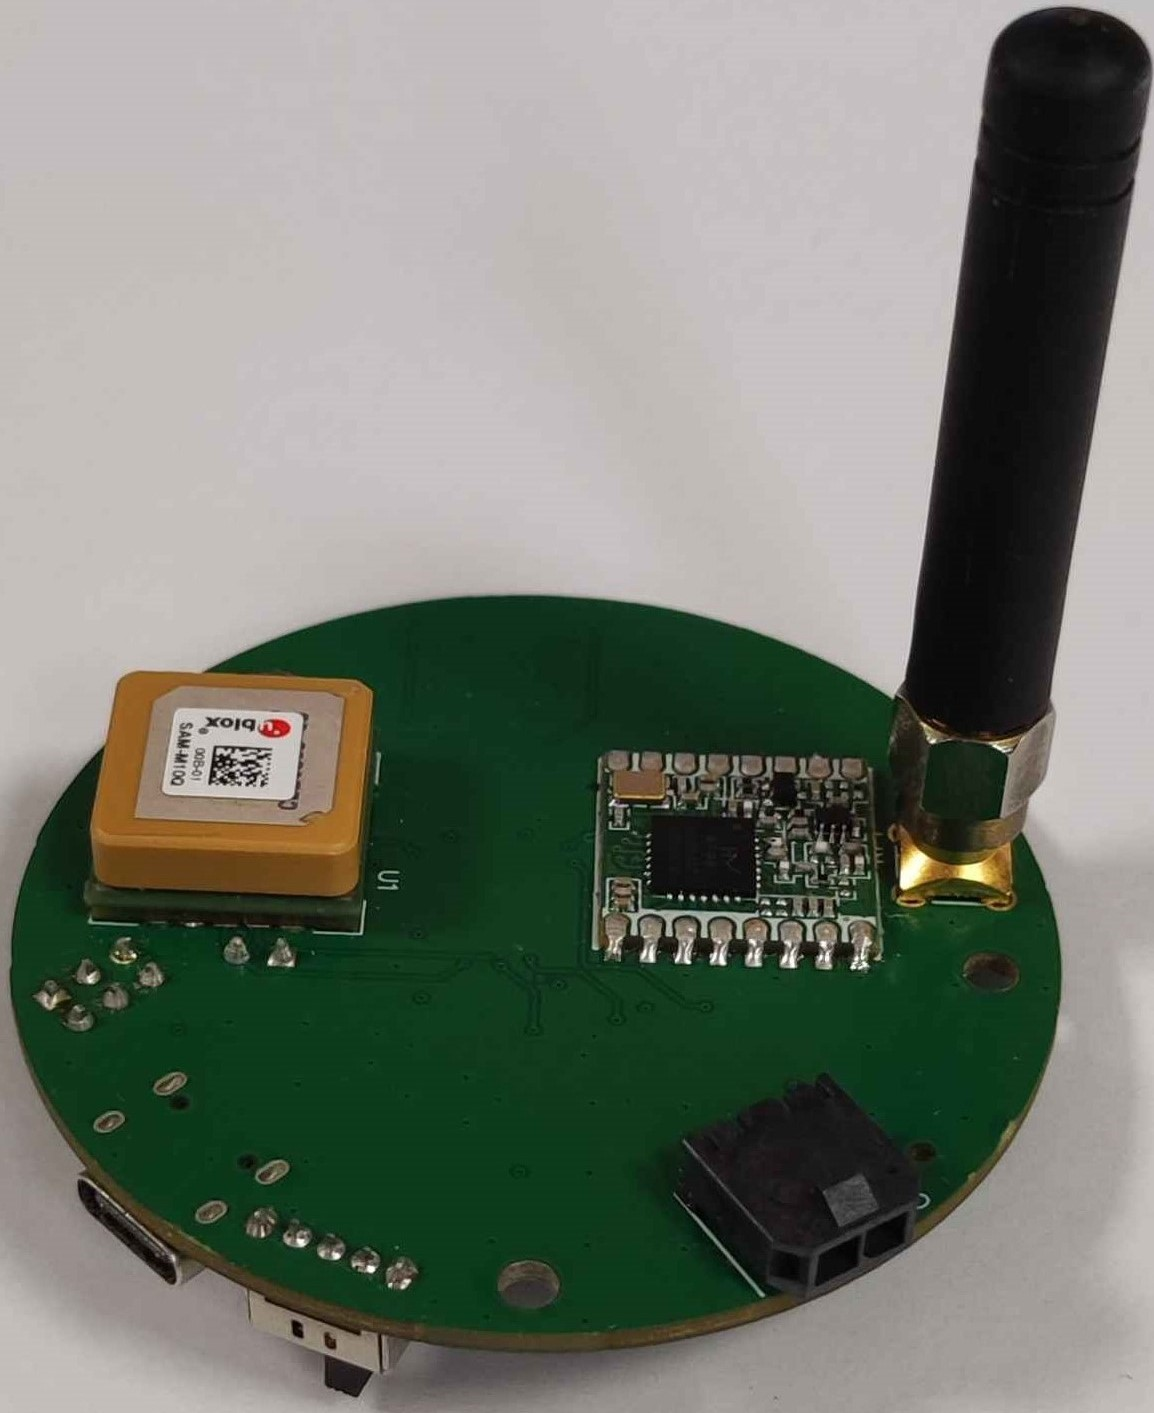
\includegraphics[width=\textwidth]{Unknown/photo/IMG_1.jpg}
        \caption{Vu de dessus}
    \end{subfigure}
    \begin{subfigure}{0.45\textwidth}
        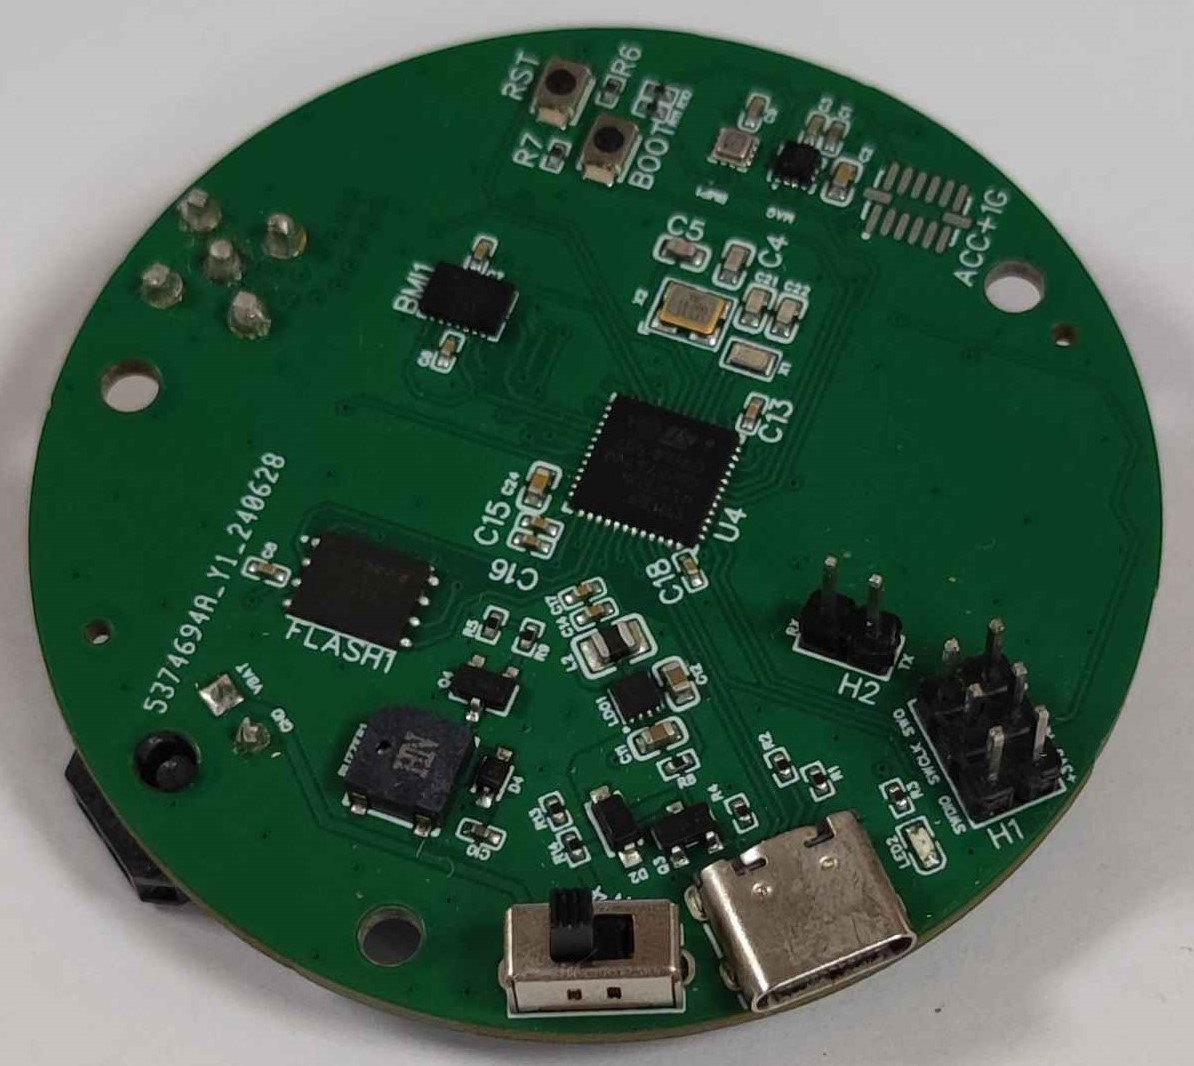
\includegraphics[width=\textwidth]{Unknown/photo/IMG_2.jpg}
        \caption{Vu de dessous}
    \end{subfigure}
    \caption{Photos du projet Unknown}
    \label{anx:fig:unknown}
\end{figure}


\end{document}
